%%%%%%%%%%%%%%%%%%%%%%%%%%%%%%%%%%%%%%%%%
% Software User Manual
% LaTeX Template
% Version 1.0 (May 1, 14)
%
% Note:
% Make sure to edit document variables in the User_Manual.cls file
%
%%%%%%%%%%%%%%%%%%%%%%%%%%%%%%%%%%%%%%%%%

%----------------------------------------------------------------------------------------
%	PACKAGES AND OTHER DOCUMENT CONFIGURATIONS
%----------------------------------------------------------------------------------------

%\documentclass[11pt, a4paper, oneside]{Manual}  % Paper size, default font size and one-sided paper
\documentclass[11pt, a4paper, twoside]{Manual}  % Paper size, default font size and two-sided paper

\usepackage{enumerate}  % The enumerate-environment is used to create numbered lists

\graphicspath{{Pictures/}}  % Specifies the directory where pictures are stored

\usepackage[square, numbers, comma, sort&compress]{natbib}  % Use the natbib reference package - read up on this to edit the reference style; if you want text (e.g. Smith et al., 2012) for the in-text references (instead of numbers), remove 'numbers'
\hypersetup{urlcolor=blue, colorlinks=true}  % Colors hyperlinks in blue - change to black if annoying
\title{\ttitle}   % Defines the thesis title - don't touch this

\begin{document}

\frontmatter  % Use roman page numbering style (i, ii, iii, iv...) for the pre-content pages

\setstretch{1.3}  % Line spacing of 1.3

% Define the page headers using the FancyHdr package and set up for one-sided printing
\fancyhead{}  % Clears all page headers and footers
\rhead{\thepage}  % Sets the right side header to show the page number
\lhead{}  % Clears the left side page header

\pagestyle{fancy}  % Finally, use the "fancy" page style to implement the FancyHdr headers

\newcommand{\HRule}{\rule{\linewidth}{0.5mm}}  % New command to make the lines in the title page

% PDF meta-data
\hypersetup{pdftitle={\ttitle}}
\hypersetup{pdfsubject=\subjectname}
\hypersetup{pdfauthor=\authornames}
\hypersetup{pdfkeywords=\keywordnames}

%----------------------------------------------------------------------------------------
%	TITLE PAGE
%----------------------------------------------------------------------------------------

\begin{titlepage}
\begin{center}

%\textsc{\LARGE \univname}\\[1.5cm]  % University name
\textsc{\Large User Manual}\\[0.5cm]  % Thesis type

\HRule \\[0.4cm] % Horizontal line
{\huge \bfseries \ttitle}\\[0.4cm]  % Thesis title
\HRule \\[1.5cm] % Horizontal line

\emph{} \\

\textsc{\Large V1.0.0}\\[2.0cm]

\href{http://theory.issp.ac.cn}{\LARGE \authornames}\\[1.5cm]  % Author name - remove the \href bracket to remove the link

\large \textit{Copyright (2014-2015) ISSP-ACS \& NSE-MIT.}\\
\large \textit{This software and manual is distributed under the GNU General Public License.}\\[5.0cm] % University requirement text
\textit{* * *}\\[0.5cm]
\groupname\\\deptname\\[0.5cm]  % Research group name and department name

{\large \today}\\[4cm] % Date
%\includegraphics{Logo}  % University/department logo - uncomment to place it

\vfill
\end{center}

\end{titlepage}

%----------------------------------------------------------------------------------------
%	DECLARATION PAGE
%	Your institution may give you a different text to place here
%----------------------------------------------------------------------------------------

\Declaration{

\addtocontents{toc}{\vspace{1em}} % Add a gap in the Contents, for aesthetics

IM3D stands for Ion Irradiation of Nanostructured Materials - a 3D Parallel Monte Carlo Simulation Code.

Copyright (2014-2015) Institute of Solid State Physics, Chinese Academy of Sciences \& Nuclear Science and Engineering, Massachusetts Institute of Technology.
This software is distributed under the GNU General Public License.
Coded by Yonggang Li (Y.G. Li), \href{ygli@theory.issp.ac.cn}{ygli@theory.issp.ac.cn}, 2014, ISSP, ACS.

\begin{itemize}

\item[\tiny{$\blacksquare$}] IM3D is a 3D Monte Carlo simulation code designed to run efficiently on serial or parallel computers. It can simulate the transport of ions and subsequent radiation damages in arbitrary complex 3D nanostructured materials.
It is an open-source code, distributed freely under the terms of the GNU Public License (GPL).

\item[\tiny{$\blacksquare$}] IM3D was sponsored by Prof. \href{http://li.mit.edu}{Ju Li} and Prof. \href{http://}{Zhi Zeng}, and mainly developed by Dr. \href{http://}{Yonggang Li} during his visiting to MIT in 2014. The supporting of CSG/FETM geometric algorithms form Prof. \href{http://http://micro.ustc.edu.cn/DingZJ/}{Zejun Ding} as well as useful contributions and discussions from Dr. Machal Short and Yang Yang are very appreciate.

\item[\tiny{$\blacksquare$}]  If you have any questions, please contact to Dr. Yonggang Li, who can be emailed at \href{ygli@theory.issp.ac.cn}{ygli@theory.issp.ac.cn}.
The IM3D Website at \href{http://}{ISSP} and \href{http://li.mit.edu/Archive/IM3D}{MIT} has more information about the code and its uses.

\end{itemize}
}

\clearpage  % Start a new page

%----------------------------------------------------------------------------------------
%	ACKNOWLEDGEMENTS
%----------------------------------------------------------------------------------------

\setstretch{1.3}  % Reset the line-spacing to 1.3 for body text (if it has changed)

\acknowledgements{\addtocontents{toc}{\vspace{1em}}  % Add a gap in the Contents, for aesthetics

This code was mainly supported by the scholarship from China Scholarship Council and Institute of Solid State Physics, Chinese Academy of Sciences (CAS) and partly by Massachusetts Institute of Technology (MIT). The subsequent supports come from the National Science Foundation of China under Grant Nos. 11275229, 11475215 \& NSAF U1230202, the Special Funds for Major State Basic Research Project of China (973) under Grant No. 2012CB933702, the Hefei Center for Physical Science and Technology under Grant No. 2012FXZY004, and Director Grants of CASHIPS. Part of the tests were performed at the Center for Computational Science of CASHIPS, the ScGrid of Supercomputing Center, and the Computer Network Information Center of the Chinese Academy of Sciences. Y.G. Li is very grateful to Prof. Xiaohong Zheng and Prof. Yongsheng Zhang for their helpful suggestions on this code and works on website design.
}
\clearpage  % Start a new page

%----------------------------------------------------------------------------------------
%	LIST OF CONTENTS/FIGURES/TABLES PAGES
%----------------------------------------------------------------------------------------

\pagestyle{fancy}  % The page style headers have been "empty" all this time, now use the "fancy" headers as defined before to bring them back

\lhead{\emph{Contents}}  % Set the left side page header to "Contents"
\tableofcontents % Write out the Table of Contents

%\lhead{\emph{List of Figures}}  % Set the left side page header to "List of Figures"
%\listoffigures  % Write out the List of Figures

%\lhead{\emph{List of Tables}}  % Set the left side page header to "List of Tables"
%\listoftables  % Write out the List of Tables

%----------------------------------------------------------------------------------------
%	ABBREVIATIONS
%----------------------------------------------------------------------------------------

%\clearpage  % Start a new page

%\setstretch{1.5}  % Set the line spacing to 1.5, this makes the following tables easier to read

%\lhead{\emph{Abbreviations}}  % Set the left side page header to "Abbreviations"
%\listofsymbols{ll}  % Include a list of Abbreviations (a table of two columns)
%{
%\textbf{LAH} & \textbf{L}ist \textbf{A}bbreviations \textbf{H}ere \\
%%\textbf{Acronym} & \textbf{W}hat (it) \textbf{S}tands \textbf{F}or \\
%}

%----------------------------------------------------------------------------------------
%	PHYSICAL CONSTANTS/OTHER DEFINITIONS
%----------------------------------------------------------------------------------------

%\clearpage % Start a new page

%\lhead{\emph{Physical Constants}} % Set the left side page header to "Physical Constants"

%\listofconstants{lrcl} % Include a list of Physical Constants (a four column table)
%{
%Speed of Light & $c$ & $=$ & $2.997\ 924\ 58\times10^{8}\ \mbox{ms}^{-\mbox{s}}$ (exact)\\
%% Constant Name & Symbol & = & Constant Value (with units) \\
%}

%----------------------------------------------------------------------------------------
%	SYMBOLS
%----------------------------------------------------------------------------------------

%\clearpage % Start a new page

%\lhead{\emph{Symbols}} % Set the left side page header to "Symbols"

%\listofnomenclature{lll} % Include a list of Symbols (a three column table)
%{
%$a$ & distance & m \\
%$P$ & power & W (Js$^{-1}$) \\
%% Symbol & Name & Unit \\

%& & \\ % Gap to separate the Roman symbols from the Greek

%$\omega$ & angular frequency & rads$^{-1}$ \\
%% Symbol & Name & Unit \\
%}

%----------------------------------------------------------------------------------------
%	DEDICATION
%----------------------------------------------------------------------------------------

%\setstretch{1.3} % Return the line spacing back to 1.3

%\pagestyle{empty} % Page style needs to be empty for this page

%\dedicatory{For/Dedicated to/To my\ldots} % Dedication text

%\addtocontents{toc}{\vspace{2em}} % Add a gap in the Contents, for aesthetics

%----------------------------------------------------------------------------------------
%	THESIS CONTENT - CHAPTERS
%----------------------------------------------------------------------------------------

\mainmatter % Begin numeric (1,2,3...) page numbering

\pagestyle{fancy} % Return the page headers back to the "fancy" style

% Include the chapters of the thesis as separate files from the Chapters folder
% Uncomment the lines as you write the chapters

% Chapter 1

\chapter{Introduction}  % Main chapter title

\label{Chapter1}  % For referencing the chapter elsewhere, use \ref{Chapter1}

\lhead{Chapter 1. \emph{Introduction}}  % This is for the header on each page - perhaps a shortened title

%----------------------------------------------------------------------------------------

This section provides an overview of what IM3D can and can't do, describe what it means for IM3D to be an open-source code.
%, and acknowledges the funding, citations and people who have contributed to IM3D during its developing.

%----------------------------------------------------------------------------------------

\section{What is IM3D}

IM3D is an open-source parallel 3D Monte Carlo (MC) code for rapidly simulating the transportation of ions and the production of defects in nanostructured materials. It is an accurate, efficient and universal 3D version of MC model developed based on the standard SRIM databases\cite{Ziegler:2010}, the fast database indexing technique\cite{Schiettekatte:2008} and MPI parallel algorithm as well as the 3D structural algorithms of Constructive Solid Geometry (CSG) / Finite Element Triangulated Mesh (FETM) methods\cite{Li:2005,Li:2008,Li:2009,Li2:2011,Zhang:2011,Li:2013}. It can model arbitrary-complex 3D targets made of different geometric elements each of which with different materials. Both the 3D distribution of ions and also all kinetic phenomena associated with the ion’s energy loss, i.e., amorphization, damage, sputtering, ionization and phonon production, can be calculated by IM3D with following all target atom cascades in detail. Thus, IM3D code provides a general and robust theoretical approach to analysis the effects in primary damage processes and the corresponding 3D space-distributions of primary defects in nanostructured materials under ion beam irradiation.
%including electronic and nuclear energy depositions, back-scatted/implanted ions, $dpa$, interstitials, vacancies and sputtering atoms, etc.

The development of IM3D is mainly includes three aspects, i.e. the accurate physical models, the universal 3D structural models and the efficient calculation algorithms. The physical parameters used in the code, such as, the electronic stopping power and energy straggling parameters, are generated from SRMModule.exe provided by SRIM package\cite{Ziegler:2010}. The 3D nanostructured samples can be generated by graphical softwares beforehand and traced by the sophisticated 3D structural algorithms based on the CSG/FETM methods\cite{Li:2005,Li:2008,Li:2009,Li2:2011,Zhang:2011,Li:2013}. In order to further increasing the efficiency of the code, we introduced the fast database indexing technique proposed in Corteo\cite{Schiettekatte:2008} to sampling the scattering and azimuthal angles as well as a linear speed-up MPI parallel algorithm or a multi-threading parallel algorithm. Detailed description of the physical basement can be found in our papers or in Appendix A.

%The ion transportation in IM3D is treated by considering an idealization of the technique principles where each %incoming ion slows down in straight line in the material until it eventually makes a collision during which it is scattered, %produces a recoil or emits a particle in a selected direction. The emitted ion also slows down along a straight trajectory %until it leaves the sample. In this idealization, the energy loss is related to the stopping power and the kinematics of the %scattering/recoiling collision. The computation of ion slowdown is carried out under three important approximations, i.e., %the binary collision approximation (BCA), the central potential approximation (CPA), and the random phase %approximation (RPA). For each collision cycle, the steps will be the determination of the flight length, the impact %parameter, the collision partner, the scattering and azimuthal angles, and, based on the latter two, of the new flying %direction. Then, the energy loss is computed, the position is incremented from the last collision locus to the new one %according to the flight length and the new flying direction, and the cycle restarts from the new collision locus until the %ion comes to rest or leaves the target. Trajectories computation helps to account as precisely as possible for the effect %of multiple collisions by reproducing in details the deviations from straight line trajectories.

IM3D can run efficiently on different platforms, including not only single- or multi-processors desktop or laptop machines but also parallel computers. Simultaneous multi-threading technique has be included in IM3D code to run on a multi-processors system. It can also run on any parallel machine that compiles plain C and supports the MPI message-passing library.

%IM3D code is developed to be an open-source code in terms of the GNU general public license[91], except for the parts of CSG/FETM models whose copyrights belong to Prof. Z.J. Ding. Thus, in order to part rights reserved, the routines related to CSG/FETM models are compiled to static libraries in IM3D package.

IM3D is a freely-available open-source code except for the geometric modules (copyrights belong to Prof. \href{http://micro.ustc.edu.cn/Members/zjding.htm}{Zejun Ding}), distributed under the terms of the GNU Public License, which means you can use or modify the code however you wish but commercial purposes. In order to part rights reserved, the routines related to CSG/FETM models are compiled to static libraries in IM3D package. In addition, a part of the modules in IM3D refer to the open-source codes, \href{http://www.nano.uni-jena.de/Forschung/Physik+mit+Ionenstrahlen/iradina-p-103.html}{Iradina}\cite{Borschel:2011} and \href{http://www.lps.umontreal.ca/~schiette/index.php?n=Recherche.Corteo}{Corteo}\cite{Schiettekatte:2008}.

%IM3D was sponsored by Prof. \href{http://li.mit.edu}{Ju Li} and developed by Dr. \href{}{Yonggang Li} when his visiting %to MIT in 2014, with the fundings mainly come from CAS and partly from MIT. Useful discussions and contributions %from Dr. Machal Short  and Yang Yang are very appreciate.

%In the most general sense, IM3D is an accurate, efficient and universal 3D Monte Carlo model developed based on the standard SRIM databases, the fast database indexing technique and MPI parallel algorithm as well as the 3D structural algorithms of CSG/FETM methods, which can provide a general and robust theoretical approach to analysis the effects in primary damage processes and the corresponding 3D space-distributions of primary defects in nanostructured materials under ion beam irradiation.

%----------------------------------------------------------------------------------------

\section{IM3D Features}

This section highlights IM3D features: %with pointers to the following sections which give more details.

\begin{itemize}

\item open-source distribution with highly portable C;
\item ion with atomic number of $1-92$ and energy of $10~eV-2~GeV/amu$, as well as different ion beam shape distribution, i.e., random, centered, defined position, random square around predefined position, Gaussian beam and etc.
\item arbitrary complex targets constructed by the 3D geometric algorithms of CSG/FETM methods\cite{Li:2005,Li:2008,Li:2009,Li2:2011,Zhang:2011,Li:2013}, with complex materials including single elements ($1-92$), alloys and compounds;
\item generate input shapes in the form of different formats (e.g. $opengl$, $ply2$ and etc.) with different standard finite element softwares, e.g. \href{http://geuz.org/gmsh/}{Gmsh}\cite{Geuzaine:2009}, \href{https://cubit.sandia.gov}{Cubit} and etc.;
\item 1D (bulk and multi-layers) or 3D systems with or without semi-infinite substrate;
\item runs from an input script or four separate input files (i.e., temp\_compfile.im3d, temp\_configfile.im3d, temp\_matfile.im3d and temp\_structfile.im3d);
\item runs on a single processor or in parallel with distributed-memory message-passing parallelism (MPI);
\item electronic energy loss and straggling are based on the standard \href{http://www.srim.org}{SRIM} databases\cite{Ziegler:2010}, and Bragg's rule\cite{Bragg:1905} is used to estimate the stopping power of a compound by the linear combination of the stopping powers of its individual elements;;
\item uses fast database indexing technique (see \href{http://www.lps.umontreal.ca/~schiette/index.php?n=Recherche.Corteo}{Corteo}\cite{Schiettekatte:2008}) or the MAGIC approximation formula \cite{Ziegler:2010} for sampling in terms of accuracy and efficiency;
\item uses the analytical modified Kinchin-Pease (KP) model\cite{Kinchin:1955,Norgett:1975} or the computationally full cascade (FC) simulation for defect generation processes;
\item uses a screened repulsive Coulomb potential described by a dimensionless screening function, such as the Thomas-Feimi potential\cite{Sommerfeld:1932}, the Lenz-Jensen potential\cite{Lenz:1932}, the Moliere potential\cite{Moliere:1947}, the Bohr potential\cite{Bohr:1948} and the universal Ziggler-Biersack-Littmark (ZBL) potential\cite{Ziegler:2010} to describe the interaction potential between two atoms;
\item output primary damage information including 1D (depth) and 3D distributions of electronic and nuclear energy depositions, back-scattering/implanted ions, $dpa$, interstitials, vacancies and sputtering atoms, etc.
\item the output distribution files are in the format of $.cfg$, $.msh$ or $.vtk$, which can be viewed by various pre- and post-processing tools such as \href{http://li.mit.edu/Archive/Graphics/A/}{AtomEye}\cite{Li:2003}, \href{http://geuz.org/gmsh/}{Gmsh}\cite{Geuzaine:2009}, \href{http://www.paraview.org/}{ParaView}, \href{https://cubit.sandia.gov/}{Cubit} and etc.

\end{itemize}

%----------------------------------------------------------------------------------------

\section{IM3D Non-features}

IM3D is designed to efficiently simulate the tracing of ions in static arbitrary complex 3D systems. Some features that IM3D does not yet (maybe in the future version) support are list below:

\begin{itemize}

\item real-time tracing plot;
\item restart;
\item 64-bit system compatibility;
\item dynamic version.

\end{itemize}

The serial version of the code can output xyz-coordinates of ions/atoms, which can give the plot of the tracing trajectories after the simulation. In the code, we introduced the fast database indexing technique (see \href{http://www.lps.umontreal.ca/~schiette/index.php?n=Recherche.Corteo}{Corteo}\cite{Schiettekatte:2008}) which is mainly based on a 32-bit system. Thus, -m32 or -arch i386 should be used in the makefile when compiling. We will also introduced a 64-bit version in the future. IM3D is a static version of the system without change the geometry shape of the system during irradiation.

Otherwise, many of the tools needed to pre- and post-process the data for 3D geometry shapes are not included in the IM3D kernel. Specifically, IM3D itself does not:

\begin{itemize}

\item run thru a GUI (would be included in the future version);
\item build 3D geometry structures;
\item perform sophisticated analyses;
\item visualize simulation results;
\item plot output data.

\end{itemize}

A few tool for constructing the input 3D geometry structures are provided as part of the IM3D package, as described in section X. Although users can be write their own tools for these tasks, but we recommend to use our tool to generate the CSG format geometry structures and the open-source software \href{http://geuz.org/gmsh/}{Gmsh} to generate the FETM format geometry structures. For high-quality visualization we recommend the \href{http://li.mit.edu/Archive/Graphics/A/}{AtomEye}\cite{Li:2003}, \href{http://geuz.org/gmsh/}{Gmsh}\cite{Geuzaine:2009} or \href{http://www.paraview.org/}{ParaView} softwares.

%----------------------------------------------------------------------------------------

\section{Open-source Distribution}

IM3D comes with no warranty of any kind. It is a copyrighted code that is distributed free-of-charge, under the terms of the \href{}{GNU Public License} (GPL). This is often referred to as open-source distribution - see \href{www.gnu.org}{www.gnu.org} or \href{www.opensource.org}{www.opensource.org} for more details. The legal text of the GPL is in the LICENSE file that is included in the IM3D distribution.

Here is a summary of what the GPL means for IM3D users:

(1) Anyone is free to use, modify, or extend IM3D in any way they choose, without including for commercial purposes.

(2) If you distribute a modified version of IM3D, it must remain open-source, meaning you distribute it under the terms of the GPL. You should clearly annotate such a code as a derivative version of IM3D.

(3) If you release any code that includes IM3D source code, then it must also be open-sourced, meaning you distribute it under the terms of the GPL.

(4) If you give IM3D files to someone else, the GPL LICENSE file and source file headers (including the copyright and GPL notices) should remain part of the code.

In the spirit of an open-source code, these are various ways you can contribute to making IM3D better. Any questions please send email to \href{ygli@theory.issp.ac.cn}{Yonggang Li (Y.G. Li)} .

%----------------------------------------------------------------------------------------

\section{Citations}

Please cite our paper if you use subroutines in this package. Thanks.

Y.G. Li, Y. Yang, M. Short, Z.J. Ding, Z. Zeng and J. Li, Fast simulation of primary damages in arbitrarily complexed nanostructured materials under ion irradiation, to be published;

Y.G. Li, Y. Yang, M. Short, Z.J. Ding, Z. Zeng and J. Li, IM3D: A 3D Parallel Monte Carlo Simulation Code for Ion Irradiation of Nanostructured Materials, to be published.

%----------------------------------------------------------------------------------------


% Chapter 2

\chapter{Getting Started}  % Main chapter title

\label{Chapter2}  % For referencing the chapter elsewhere, use \ref{Chapter1}

\lhead{Chapter 2. \emph{Getting Started}}  % This is for the header on each page - perhaps a shortened title

%----------------------------------------------------------------------------------------

This section describes how to build and run IM3D.

%----------------------------------------------------------------------------------------

\section{What is in the IM3D Distribution}

When you download IM3D you will need to unzip and untar the downloaded file with the following commands, after placing the file in an appropriate directory.

\quad \textsl{gunzip im3d*.tar.gz}

\quad \textsl{tar xvf im3d*.tar}

This will create an IM3D directory containing two files and several sub-directories:

\begin{itemize}

\item README ~~~~~ Text file, general information;

\item LICENSE ~~~~~ The GNU General Public License (GPL);

\item bin ~~~~~~~~~~~~~~ Executable files;

\item data ~~~~~~~~~~~~~ SRIM databases, input indexing tables, material properties, etc.;

\item doc ~~~~~~~~~~~~~~ User manual;

\item examples ~~~~~~ Tests and examples;

\item lib ~~~~~~~~~~~~~~~ Static libraries used for IM3D code, geometric modules.

\item src ~~~~~~~~~~~~~~~ Source codes;

\item tools ~~~~~~~~~~~~ Useful tools for generating input script, shapes, databases and etc.

\end{itemize}

%----------------------------------------------------------------------------------------

\section{Making IM3D}

\subsection{Steps to build an IM3D executable file}

Systems:
    $Windows$, $Linux$ or $Mac$.

Compiler:
    Microsoft Visual Studio - $c$ / $mingw32$, $gcc$ and etc.

Libraries \& packages:
    Standard $C$ library and $MPICH$ / $OpenMP$ package.


The src directory contains the plain C source and header files for IM3D. It also contains a makefile file for linux/Mac systems:

\# This makefile can be used to compile im3d.\\
\# On Linux/UNIX or Mac systems, gcc is recommend for compilation.\\
\# On Windows system, mingw32 is recommend for compilation.

\#CC = gcc \# serial, linux or Mac\\
\#CC = mingw32-gcc \# serial, win\\
CC = mpicc \# mpi, linux or Mac

\#CFLAGS = -O2 -Wall -ansi -pedantic\\
\#CFLAGS = -O2 -Wall -pedantic\\
\#CFLAGS = -O1 -Wall\\
CFLAGS = -O1 -Wall -m32 \# for 64-bit systems, -m32 or -arch i386 must be included\\
LDFLAGS = -lm -m32 \# for 64-bit systems, -m32 or -arch i386 must be included\\
\#LIBFLAG = -L. -lstruct\_s \# include static library, serial\\
LIBFLAG = -L. -lstruct\_m \# include static library, mpi

\# Notes on warning level:\\
\# Using -Wall and -pedantic will return many warnings, because of non-allowed\\
\# comment styles in the codes. I recommend using just -Wall.

\# Notes on the compiler optimization options -OX:\\
\# It is not recommended to use -O2 or -O3. On Linux systems no problems using\\
\# these options have been observed so far; however, on windows systems porgram\\
\# crashes and hang-ups did occur when using -O2 or -O3.\\
\# In windows, the inverse sqr tables will not work with -O2.\\
\# If unsure, compile all with -O1 only.

im3d \: im3d.o mpimod.o const.o init.o material.o target.o matrix.o index.o magic.o fileio.o cfgwriter.o mshwriter.o bulk.o utils.o random.o\\
  \$(CC) \$(LDFLAGS) -o iran3d im3d.o mpimod.o const.o init.o material.o target.o matrix.o index.o magic.o fileio.o cfgwriter.o mshwriter.o bulk.o utils.o random.o \$(LIBFLAG)

im3d.o: im3d.h im3d.c

mpimod.o: mpimod.h mpimod.c

const.o: const.h const.c

init.o: init.h init.c

material.o: material.h material.c

target.o: target.h target.c

matrix.o: matrix.h matrix.c

index.o: index.h index.c

magic.o: magic.h magic.c

fileio.o: fileio.h fileio.c

cfgwriter.o: cfgwriter.h cfgwriter.c

mshwriter.o: mshwriter.h mshwriter.c

bulk.o: bulk.h bulk.c

utils.o: utils.h utils.c

random.o: random.h random.c

.c.o :\\
	\$(CC) -c \$(CFLAGS) \$$<$

clean:\\
	rm -f iran3d *.o

clear:\\
	rm *.o

Then, you can just type "make" to compile the code:

\quad \textsl{make}

Finally, an executable file "im3d" should be generated when the build is complete.

\subsection{Command switch}

The geometry modules are not open-source but can be called in the terms of static libraries, that is

\quad \textsl{struct\_s.a, struct\_m.a.}

where s and m denote as serial and parallel version of the libraries, respectively. Thus, please switch 'LIBFLAG = -L. -lstruct\_s' to 'LIBFLAG = -L. -lstruct\_m', when use the MPI parallel version.

\subsection{Errors that can occur when making IM3D}

Link errors: all of the libraries used in makefile should be 32-bit version, including $gcc$ and $mpich$ libraries, etc.
%----------------------------------------------------------------------------------------

\section{Runing IM3D}

IM3D can be run from a command-line options in a serial computer or a MPI parallel super computer.

serial-single-thread:

\quad \textsl{./im3d -command}

serial-multi-threads:

\quad \textsl{./multithread.sh}

MPI parallel:

\quad e.g., \textsl{mpirun -n \$cpu ./im3d -command}

%----------------------------------------------------------------------------------------

\section{Command-line Options}

IM3D can be run from a command line, so that you can check the output. If no parameters are provided, IM3D assumes that there is a configuration file named Config.in in the current directory and loads the configuration from this file. However, you can provide various command line arguments (they are all optional):

\begin{itemize}
\item[] -h                       \quad Prints the help (basically like this table).
\item[] -l                        \quad Display the license file.
\item[] -c FILENAME    \quad Instructs IM3D to use FILENAME as the configuration file instead of the default Config.in.
\item[] -p NUMBER      \quad Specify how much info to print to console. -2 means very little, 2 means a lot, with various possibilities in between.
\item[] -n NUMBER      \quad Default is 0. Specifies how many ions are simulated (overrides the setting speci- fied in the config file).
\item[] -E NUMBER      \quad Sets the energy of the ions. This option overrides the setting from the config file.
\item[] -w                      \quad Wait for return key before exiting (useful if started from another program and you still want to see output).
\item[] -m -d                 \quad Do not simulate anything, only estimate memory usage (roughly). Print details for memory usage (only useful when -m option also supplied).
\item[] -g STRING        \quad Generate and update status file while running. See details below.
\end{itemize}

The program mostly does not check whether the input parameters make any sense. In case some parameters are missing or completely out of range, the program will most likely crash or create strange results.

The -g option is useful when letting IM3D do background work for other programs. It instructs IM3D to output its current status to a file, which can be monitored by other programs (for example by a user interface). If it is set, every 200 ions IM3D writes exactly four lines to the file ir{\_}state.dat. The first line contains the word IM3D and the version of IM3D. The second line contains the string submitted on the command line after the -g option. The third line contains a status word. The fourth line contains the number of ions that have been simulated. The status words and their meanings are:

\begin{itemize}
\item[] init0 \quad IM3D has started.
\item[] init1 \quad The config files have been read.
\item[] init2 \quad Everything is initialized and ready.
\item[] sim \quad Simulation is running.
\item[] simend \quad Simulation has finished.
\item[] end \quad Simulation results have been stored and IM3D will terminate immediately.
\end{itemize}

%----------------------------------------------------------------------------------------

\section{IM3D Screen Output}

As IM3D reads an input script, it prints information to the screen about significant actions it tanks to setup a simulation. When the simulation is ready to begin, IM3D performs various initializations and prints the feed-back information. It also prints the details of the initial geometry structure of the system. During the run itself, completed status is printed periodically, every constant ions numbers. When the run concludes, IM3D appends statistics about the CPU time approximately. An example set of the screen output is shown here:

************************************************************************\\
IM3D: Ion IRadiation of Nanostructured materials\\
        -- a 3D parallel Monte Carlo simulation code\\
\\
IM3D Version 1.0.0, Apr. 29th, 2014\\
 -- \\
by Yonggang Li (Y.G. Li), 2014, ygli@theory.issp.ac.cn \& ygli@mit.edu;\\
Institute of Solid Status of Physics, Chinese Academy of Sciences;\\
\& Nuclear Science and Engineering, Massachusetts Institute of Technology.\\
\\
Refers to:\\
  H.M. Li, H.Y. Wang, Y.G. Li \& Z.J. Ding*'s CSG/FETM geometry methods;\\
\& C. Borschel's OSS 'iradina' and F. Schiettekatte's OSS 'corteo'.\\
\\
This program comes with ABSOLUTELY NO WARRANTY.\\
This is free software, and you are welcome to redistribute it under\\
certain conditions, see LICENCE for details.\\
************************************************************************\\
\\
Seed in node 2 is: 39419295	93145296\\
Seed in node 1 is: 39419294	93145295\\
Seed in node 3 is: 39419296	93145297\\
Seed in node 0 is: 39419293	93145294\\
Configuration read from temp\_configfile.im3d.\\
Corteo scattering matrix loaded.\\
Lists of random numbers generated.\\
Chu's straggling data read.\\
Invsere Erf list read.\\
Invsere Erf list randomized.\\
Prepare scattering matrices for ion on target collisions... finished\\
Prepare scattering matrices for recoil on target collisions...\\
i: 0; my\_shape:  1; is\_full:   1\\
i: 1; my\_shape:  2; is\_full:   1\\
i: 2; my\_shape:  3; is\_full:   1\\
i: 3; my\_shape:  4; is\_full:   1\\
i: 4; my\_shape:  5; is\_full:   1\\
i: 5; my\_shape:  6; is\_full:   1\\
i: 6; my\_shape:  7; is\_full:   1\\
i: 7; my\_shape:  8; is\_full:   1\\
i: 8; my\_shape:  9; is\_full:   1\\
z0\_max\_csg: 101 (nm), must larger than the max depth of goemetry structure!\\
i: 0; my\_shape:  1; is\_full:   1\\
i: 1; my\_shape:  2; is\_full:   1\\
i: 2; my\_shape:  3; is\_full:   1\\
i: 3; my\_shape:  4; is\_full:   1\\
i: 4; my\_shape:  5; is\_full:   1\\
i: 5; my\_shape:  6; is\_full:   1\\
i: 6; my\_shape:  7; is\_full:   1\\
i: 7; my\_shape:  8; is\_full:   1\\
i: 8; my\_shape:  9; is\_full:   1\\
z0\_max\_csg: 101 (nm), must larger than the max depth of goemetry structure!\\
 finished\\
Materials read from temp\_matfile.im3d.\\
Initializing target.\\
Target structure definition file: temp\_structfile.im3d\\
\\
Target size is: \\
x: 60 cells, 10 nm per cell, 600 nm in total.\\
y: 60 cells, 10 nm per cell, 600 nm in total.\\
z: 20 cells, 5 nm per cell, 100 nm in total.\\
Total: 72000 cells in 3.6e+07 nm\^3.\\
----------------------------------------------\\
i: 0; my\_shape:  1; is\_full:   1\\
  Solid Sphere:\\
    Radius(nm):   50.000\\
    Center(nm):  100.000  100.000   50.000\\
i: 1; my\_shape:  2; is\_full:   1\\
  Solid Tetrahedrona:\\
Vertex(nm):    300.000    110.000      0.100\\
               300.000     50.000    100.000\\
               250.000    140.000    100.000\\
               350.000    140.000    100.000\\
i: 2; my\_shape:  3; is\_full:   1\\
  Solid Cuboid:\\
     Vertex(nm): \\
    450.000     50.000      0.000 \\
Side Length(nm): \\
    100.000    100.000    100.000 \\
    Orientation: \\
      1.000      0.000      0.000 \\
      0.000      1.000      0.000 \\
      0.000      0.000      1.000 \\
i: 3; my\_shape:  4; is\_full:   1\\
  Solid Ellipsoid:\\
    Semi-axes(nm): \\
      75.000   50.000   40.000\\
    Shift(nm):  100.000  300.000   50.000\\
i: 4; my\_shape:  5; is\_full:   1\\
  Solid Taper:\\
    Vertex Angle(D):   30.000\\
         Height(nm):   80.000\\
    Shift(nm):  300.000  300.000    0.100\\
i: 5; my\_shape:  6; is\_full:   1\\
  Solid Column:\\
    Radius(nm):   50.000\\
    Height(nm):  100.000\\
    Shift(nm):  500.000  300.000    0.000\\
i: 6; my\_shape:  7; is\_full:   1\\
  Solid Polyhedron:\\
  6\\
   4\\
  50.000  425.000  100.010\\
  50.000  575.000  100.010\\
  59.963  575.000    0.000\\
  59.963  425.000    0.000\\
   4\\
  59.963  425.000    0.000\\
  59.963  575.000    0.000\\
 144.963  575.000    0.000\\
 144.963  425.000    0.000\\
   4\\
 144.963  425.000    0.000\\
 144.963  575.000    0.000\\
 154.926  575.000  100.010\\
 154.926  425.000  100.010\\
   4\\
  50.000  425.000  100.010\\
  50.000  575.000  100.010\\
 154.926  575.000  100.010\\
 154.926  425.000  100.010\\
   4\\
  50.000  425.000  100.010\\
  59.963  425.000    0.000\\
 144.963  425.000    0.000\\
 154.926  425.000  100.010\\
   4\\
  50.000  575.000  100.010\\
  59.963  575.000    0.000\\
 144.963  575.000    0.000\\
 154.926  575.000  100.010\\
i: 7; my\_shape:  8; is\_full:   1\\
  Solid Paraboloid:\\
    Radius(nm):   50.000\\
    Height(nm):  100.000\\
    Shift(nm):  300.000  500.000    0.000\\
i: 8; my\_shape:  9; is\_full:   1\\
  Solid Hyperboloid:\\
    Distance(nm):   20.000\\
      Radius(nm):   50.000\\
      Height(nm):   80.000\\
    Shift(nm):  500.000  500.000    0.000\\
z0\_max\_csg: 101 (nm), must larger than the max depth of goemetry structure!\\
----------------------------------------------\\
This is the CSG geometry version of im3d.\\
\\
Target composition read from temp\_compfile.im3d.\\
Target structure read from temp\_structfile.im3d.\\
Normalization factor:	1\\
\\
Starting simulation of irradiation...\\
i: 0; my\_shape:  1; is\_full:   1\\
i: 1; my\_shape:  2; is\_full:   1\\
i: 2; my\_shape:  3; is\_full:   1\\
i: 3; my\_shape:  4; is\_full:   1\\
i: 4; my\_shape:  5; is\_full:   1\\
i: 5; my\_shape:  6; is\_full:   1\\
i: 6; my\_shape:  7; is\_full:   1\\
i: 7; my\_shape:  8; is\_full:   1\\
i: 8; my\_shape:  9; is\_full:   1\\
z0\_max\_csg: 101 (nm), must larger than the max depth of goemetry structure!\\
Completed: 0\%\\
Completed: 0.8\%\\
Completed: 1.6\%\\
...\\
...\\
...\\
Completed: 97.6\%\\
Completed: 98.4\%\\
Completed: 99.2\%\\
Storing final results: ...\\
 done.\\
\\
Run time: 71.000000 seconds.

%----------------------------------------------------------------------------------------



% Chapter 3

\chapter{Input}  % Main chapter title

\label{Chapter3}  % For referencing the chapter elsewhere, use \ref{Chapter1}

\lhead{Chapter 3. \emph{Input}}  % This is for the header on each page - perhaps a shortened title

%----------------------------------------------------------------------------------------

\section{IM3D Input Script}

IM3D input script is in the $iradina$ format, which reads the input from four input files: the first file is a general configuration file describing how the program is supposed to run (contains mostly simulation parameters etc.). The second file describes the material properties of all materials found in the target. The third file defines the structure of the simulation volume. The fourth file holds the description of the 3D target (i.e. the shapes of CSG or FETM nanosized object).

The first three files look similar to other configuration file types (and are mostly human-readable): empty lines or lines starting with a \#–sign are ignored. All other lines can either denote the beginning of a new section by [section name] or can contain a parameter definition: parname=value(s). Note that omitting any parameter might result in undefined behavior or crashes of the program. Upper and lower case letters cannot be exchanged! Recommendation: Use existing example files and adapt them according to your needs.

Alternatively, it is possible to put all the information from the four input files into one combined input file (Config.in), see details in section 3.1.5.

%----------------------------------------------------------------------------------------

\section{Input Script Structure}

\subsection{Configuration File: temp\_configfile.im3d}

The contents of the configuration file will be explained line-by-line. Detailed explanations can be found in $gen\_config$ tool (./tool/gen\_configs).

\begin{enumerate}[1:~]
\item \# Configuration file for im3d

\item ~[IonBeam]
\item max\_no\_ions=50000

\# the number of protons of the ion, range of $(1, 10^8)$, generally $10^5$ is enough and recommended;

\item ion\_Z= 14

\# the mass in atomic mass units, range of $(1, 92)$;

\item ion\_M=28.0

\# the atomic weight of ion;

\item ion\_E0=50000

\# the primary energy of the ion in unit of eV, range of $(10 eV, 2 GeV)$;

\item ion\_vx=0
\item ion\_vy=0
\item ion\_vz=1

\# the incident direction (vx, vy, vz) of the ion; range of $(0, 1)$;

\item ion\_distribution=0

\# the distribution type of the ion: 0-random, 1-centered, 2-defined position, 3-random square around predefined position, 4-Gaussian beam, sigma = bean\_spread;

\item enter\_x=20
\item enter\_y=20
\item enter\_z=-10

\# the enter position $(x, y, z)$ of ions when random beam is note selected, $z$ must be higher than the target;

\item beam\_spread=1.5

\# the spread of the beam in $xy$-space for Gaussian beam;

\item ~[Simulation]
\item OutputFileBaseName=./output/

\# output path, ./output/ is selected in default;

\item output\_format=1

\# output\_file format: 0-iradina, 1-cfg, 2-msh, 3-vtk;

\item normalize\_output=0

\# normalize output results or not;

\item display\_interval=100

\# the interval of display, range of $(1, max\_no\_ions)$;

\item storage\_interval=1000

\# the storage of display, range of $(1, max\_no\_ions)$;

\item store\_transmitted\_ions=0

\# store transmitted ions or not;

\item store\_exiting\_recoils=0

\# store existing recoils or not;

\item store\_exiting\_limit=100

\# the maximum number of exiting recoils to be stored;

\item store\_energy\_deposit=1

\# array with deposited energy are created and stored or not;

\item store\_ion\_paths=0

\# store the exact ion paths or not, =1 only for the serial version;

\item store\_path\_limit = 100;

\# the maximum number of stored paths, range of $(1, 1000)$ is recommended, =-1 when store\_ion\_paths=0;

\item transport\_type=1

\# transport type, =0 full and accurate projectile transport, =1 fast projectile transport;

\item multiple\_collisions=1

\# the maximum number of multiple collisions, 0 means just 1;

\item flight\_length\_type=0

\# the flight length type: 0->Random Poisson dist., 1->Constant;

\item flight\_length\_constant=0.3

\# if flight\_length\_type=1, set its flight\_length\_constant;

\item scattering\_calculation=0

\# the scattering calculation type: 0->SRIM-Corteo database, 1->MAGIC approximation;

\item tracing\_recoil\_or\_not=1

\# tracing the exact recoils cascades or not, 0-KP, 1-FC;

\item store\_recoil\_cascades=0

\# store the exact recoils cascades or not;

\item detailed\_sputtering=1

\# detailed calculation of sputtering or not;

\item single\_ion\_sputter\_yields=0

\# if detailed\_sputtering=1, store sputter yields for single ions or not;

\item do\_not\_store\_damage=0

\# store damages or not;

\item min\_energy=5

\# the minimum energy below which all projectiles are stopped, range of $(0, ion\_E0)$;

\item seed1=39419293
\item seed2=93145294

\# random seeds, 8-digit integers.

\item ~[Target]
\item geometry\_type=1

\# the geometry type: 0->bulk, 1->csg, 2->fetm;

\item no\_substrate=1

\# with substrate or not;

\item gen\_shape\_or\_not=1

\# if geometry\_type == 2, generate fetm shape from ply2 file by IM3D or pre-generated fetm shape by triangle.f90 code;

\item straggling\_model=3

\# the straggling model: 0->No straggling, 1->Bohr, 2->Chu, 3->Chu+Yang;

\item MaterialsFileName=Materials.in

\# filename that defines the materials in the target, in default;

\item TargetstructureFileName=Structure.in

\# filename that define the structure of the target, in default.

\end{enumerate}

\subsection{Materials File: temp\_matfile.im3d}

\begin{enumerate}[1:~]
\item ~[GaAs]

\# name;

\item element\_count=2

\# the number of elements in the material;

\item density=4.43e22

\# the density of the material;

\item elements\_Z=31,33

\# the atomic numbers of the elements in the material;

\item elements\_M=69.72,74.92

\# the atomic weights of the elements in the material;

\item elements\_conc=0.5,0.5

\# the atomic contents of the elements in the material;

\item elements\_dispEnergy=20.0,25.0

\# the displacement energies of the elements in the material;

\item elements\_latt\_energy=3.0,3.0

\# the bulk lattice energies of the elements in the material;

\item elements\_surf\_energy=2.0,1.2

\# the surface lattice energies of the elements in the material;

\item ion\_surf\_energy=2.0

\# the surface lattice energies of the ion in the material.

\end{enumerate}

\subsection{Structure File: temp\_structfile.im3d}

\begin{enumerate}[1:~]
\item \# Structure definition file for im3d

\item ~[Target]
\item cell\_count\_x=60
\item cell\_count\_y=60
\item cell\_count\_z=20

\# the numbers of cells along $(x, y, z)$-axis, respectively;

\item cell\_size\_x=10
\item cell\_size\_y=10
\item cell\_size\_z=5

\# the intervals of cells along $(x, y, z)$-axis, respectively;

\item sub\_surf\_z=101

\# the z-position of the substrate surface;

\item CompositionFileType=0

\# only used for iradina file type: 0->one column, 1->four column;

\item CompositionFileName=testwire.conc.in

\# filename that defines the composition in the target, in default.

\end{enumerate}

\subsection{Composition File: temp\_compfile.im3d}

IM3D has two different types of composition files related to $CSG$ and $FETM$ methods, respectively. 

For CSG method, explanations can be found in in $gen\_config$ tool (./tool/gen\_configs) in detail. In the composition file it includes:

~1~~~~~~~~\# Sphere\\
~~1\\
~100.000~100.000~~50.000~~50.000\\
~~0\\
~~0\\
~2~~~~~~~~\# Tetrahedron\\
~~1\\
~300.000~110.000~~~0.100\\
~300.000~~50.000~100.000\\
~250.000~140.000~100.000\\
~350.000~140.000~100.000\\
~~0\\
~~0\\
~3~~~~~~~~\# Cuboid\\
~~1\\
~450.000~~50.000~~~0.000\\
~100.000~100.000~100.000\\
~~~1.000~~~0.000~~~0.000\\
~~~0.000~~~1.000~~~0.000\\
~~~0.000~~~0.000~~~1.000\\
~4~~~~~~~~\# Ellipsoid\\
~~1\\
~~75.000~~50.000~~40.000\\
~-1\\
~100.000~300.000~~50.000\\
~~0\\
~~0\\
~~0\\
~5~~~~~~~~\# Taper\\
~~1\\
~~30.000~~80.000\\
~-1\\
~300.000~300.000~~~0.100\\
~~0\\
~~0\\
~~0\\
~6~~~~~~~~\# Column\\
~~1\\
~~50.000~100.000\\
~-1\\
~500.000~300.000~~~0.000\\
~~0\\
~~0\\
~~0\\
~7~~~~~~~~\# Polyhedron\\
~~1\\
~~6\\
~~~4\\
~~50.000~425.000~100.010\\
~~50.000~575.000~100.010\\
~~59.963~575.000~~~0.000\\
~~59.963~425.000~~~0.000\\
~~~4\\
~~59.963~425.000~~~0.000\\
~~59.963~575.000~~~0.000\\
~144.963~575.000~~~0.000\\
~144.963~425.000~~~0.000\\
~~~4\\
~144.963~425.000~~~0.000\\
~144.963~575.000~~~0.000\\
~154.926~575.000~100.010\\
~154.926~425.000~100.010\\
~~~4\\
~~50.000~425.000~100.010\\
~~50.000~575.000~100.010\\
~154.926~575.000~100.010\\
~154.926~425.000~100.010\\
~~~4\\
~~50.000~425.000~100.010\\
~~59.963~425.000~~~0.000\\
~144.963~425.000~~~0.000\\
~154.926~425.000~100.010\\
~~~4\\
~~50.000~575.000~100.010\\
~~59.963~575.000~~~0.000\\
~144.963~575.000~~~0.000\\
~154.926~575.000~100.010\\
~8~~~~~~~~\# Paraboloid\\
~~1\\
~~50.000 100.000\\
~-1\\
~300.000~500.000~~~0.000\\
~~0\\
~~0\\
~~0\\
~9~~~~~~~~\# Hyperboloid\\
~~1\\
~~20.000~~50.000~~80.000\\
~-1\\
~500.000~500.000~~~0.000\\
~~0\\
~~0\\
~~0\\
~0\\
~0.0\\

For FETM method, in the composition file it includes:

50.0~~50.0~~122.0~~~~~~~~\# box\_start\_x0, box\_start\_y0, box\_start\_z0;\\
11~~11~~11~~~~~~~~~~~~~~~\# box\_count\_x,  box\_count\_y,  box\_count\_z ;\\
10.1~~10.1~~10.1~~~~~~~~~\# box\_size\_x,   box\_size\_y,   box\_size\_z  ;\\
\# space subdivision for FETM targets;\\
2~~~~~~~~~~~~~~~~~~~~~~~~\# file format, 1-file1.dat generated by opengl, 2-file1.ply2 generated by Gmsh;\\
1~~~~~~~~~~~~~~~~~~~~~~~~\# the number of materials or file1s;\\
1~~12~~~~~~~~~~~~~~~~~~~~\# material\_type, number\_of\_data\\
100.0~~100.0~~100.0~~~~~~\# the scaling of the target, scaling\_x, scaling\_y, scaling\_z;\\
0.0~~0.0~~0.0~~~~~~~~~~~~\# the transformation of the target, trans\_x, trans\_y, trans\_z.\\

And in another input file (file1.ply2), shapes are described like (take a cube as example):

8\\
12\\
0 0 0\\
1 0 0\\
0 1 0\\
1 1 0\\
0 0 1\\
1 0 1\\
0 1 1\\
1 1 1\\
3 0 1 3\\
3 0 2 3\\
3 0 4 6\\
3 0 2 6\\
3 0 1 5\\
3 0 4 5\\
3 2 6 3\\
3 6 7 3\\
3 1 3 5\\
3 3 5 7\\
3 5 6 7\\
3 4 5 6\\

\subsection{Combined Input File}

You can also put all the information from the four input files into one combined input file, i.e., Config.in. Before running, Config.in will automatically spits into four temporary input files: temp\_configfile.im3d, temp\_matfile.im3d, temp\_structfile.im3d and temp\_compfile.im3d.
%----------------------------------------------------------------------------------------

% Chapter 4

\chapter{Output}  % Main chapter title

All of output files can be found in the path of

\quad \textsl{./output/}.

\label{Chapter4}  % For referencing the chapter elsewhere, use \ref{Chapter1}

\lhead{Chapter 1. \emph{Output}}  % This is for the header on each page - perhaps a shortened title

%----------------------------------------------------------------------------------------

\section{List of Output Files}

In the output path, there would be a list of output files as defined in input script, i.e.,

\begin{itemize}

\item aiv.xyz.cfg

\item cascades

\item depth\_dist\_functions.dat

\item disp.mat$*$.cfg, disp.mat$*$.msh or disp.mat$*$.vtk

\item energy.deposit.cfg, energy.deposit.msh or energy.deposit.vtk

\item int.mat$*$.cfg, int.mat$*$.msh or int.mat$*$.vtk

\item ion\_paths

\item ions.replacements.cfg, ions.replacements.msh or ions.replacements.vtk

\item ions.total.cfg, ions.total.msh or ions.total.vtk

\item leaving.mat$*$.cfg, leaving.mat$*$.msh or leaving.mat$*$.vtk

\item leaving\_directions.ions

\item leaving\_directions.sum

\item leaving\_directions.z$*1$.m$*2$.mat$*3$.elem$*4$

\item radial\_dist\_functions.dat

\item repl.mat$*$.cfg, repl.mat$*$.msh or repl.mat$*$.vtk

\item transmitted.ions

\item vac.mat$*$.cfg, vac.mat$*$.msh or vac.mat$*$.vtk

\end{itemize}

\subsection{aiv.xyz.cfg}

$aiv.xyz.cfg$ is an output file of the detailed position of ions and defects generated in materials, which includes 7 columns, i.e., x, y, z, defect type, defect belong to which ion, material and element. It is in the format of .cfg at present and can be viewed by AtomEye software directly. An example of this output file is list below:

Number of particles = 801809\\
A = 10 Angstrom (basic length-scale)\\
H0(1,1) = 1000 A\\
H0(1,2) = 0.0 A\\
H0(1,3) = 0.0 A\\
H0(2,1) = 0.0 A\\
H0(2,2) = 1000 A\\
H0(2,3) = 0.0 A\\
H0(3,1) = 0.0 A\\
H0(3,2) = 0.0 A\\
H0(3,3) = 1000 A\\
.NO\_VELOCITY.\\
entry\_count = 7\\
auxiliary[0] = type (A-I-V)\\
auxiliary[1] = tab (A-ion)\\
auxiliary[0] = mater\\
auxiliary[1] = element\\
4\\
aiv\_pos\\
0.500743	0.500435	0.001079	2	0	1	0\\
0.500792	0.500568	0.001067	1	0	1	1\\
0.500740	0.500452	0.001087	2	0	1	1\\
0.500473	0.501270	0.001831	1	0	1	0\\
0.500484	0.500152	0.001079	2	0	1	0\\
0.500476	0.499380	0.001042	1	0	1	1\\
...         ...         ...         .   .   .   .

\subsection{Output: cascades}

\subsection{Output: depth\_dist\_functions.dat}

\subsection{Output: disp.mat$*$.cfg/.msh/.vtk}

\subsection{Output: energy.deposit.cfg/.msh/.vtk}

\subsection{Output: int.mat$*$.cfg/.msh/.vtk}

\subsection{Output: ion\_paths}

\subsection{Output: ions.replacements.cfg/.msh/.vtk}

\subsection{Output: ions.total.cfg/.msh/.vtk}

\subsection{Output: leaving.mat$*$.cfg/.msh/.vtk}

\subsection{Output: leaving\_directions.ions}

\subsection{Output: leaving\_directions.sum}

\subsection{Output: leaving\_directions.z$*1$.m$*2$.mat$*3$.elem$*4$}

\subsection{Output: radial\_dist\_functions.dat}

\subsection{Output: repl.mat$*$.cfg/.msh/.vtk}

\subsection{Output: transmitted.ions}

\subsection{Output: vac.mat$*$.cfg/.msh/.vtk}

%----------------------------------------------------------------------------------------

\section{Output Format}

Three types of output formats are given in IM3D code till now, including $.cfg$, $.msh$ and $.vtk$.

\subsection{$.cfg$ format}


\subsection{$.msh$ format}


\subsection{$.vtk$ format}


%----------------------------------------------------------------------------------------

\section{Output Visualization}

Different kinds of softwares can be feasibly used to visualize the 3D distributions of primary defects in output files, such as, \href{http://li.mit.edu/Archive/Graphics/A/}{AtomEye}, \href{http://geuz.org/gmsh/}{Gmsh} and \href{http://www.paraview.org/}{ParaView}, etc. AtomEye software is a easy tool to quickly visualize the $.cfg$ format files. While for much higher qualities, Gmsh or ParaView is commented to be used with the output files in the formats of $.msh$ and $.vtk$, respectively.

%----------------------------------------------------------------------------------------


% Chapter 5

\chapter{Accelerating IM3D Performance}  % Main chapter title

\label{Chapter5}  % For referencing the chapter elsewhere, use \ref{Chapter1}

\lhead{Chapter 5. \emph{Accelerating IM3D Performance}}  % This is for the header on each page - perhaps a shortened title

%----------------------------------------------------------------------------------------

\section{General Strategies}

In order to further increasing the efficiency of the code, we introduce the fast database indexing technique proposed by Schiettekatte in Corteo code\cite{Schiettekatte:2008} to sampling the scattering and azimuthal angles and the stopping powers as well as two numerical acceleration algorithms to implement parallel computing.

%----------------------------------------------------------------------------------------

\section{Fast Database Indexing Techniques}

For the calculation of the classical binary atomic scattering angle, IM3D code thus introduce the fast routines from Corteo which are based on both the fast indexing technique and the MAGIC approximation\cite{Ziegler:2010} alternatively in terms of accuracy, efficiency and memory usage. For the calculation of the stopping power, the same algorithm of computing the classical binary atomic scattering angle can also be used by firstly generating the tables of stopping power values and directly finding a desired value form these tables in use.
%The fast indexing technique naturally have the advantage of high efficiency for determining the scattering angles comparing to MAGIC algorithm, but nearly without reducing of accuracy.
For the case of the number of elements included in a target is not too big, the memory burden is no more than several MB. The detailed treatment of the fast indexing techniques can be found in Ref.\cite{Borschel:2011,Schiettekatte:2008}.

\subsection{}


\subsection{}


\subsection{}


%----------------------------------------------------------------------------------------

\section{MPI Parallel and Multi-threading}

Furthermore, in order to further enhance the computational efficiency, the MPI parallel and multi-threading methods have been integrated into IM3D code. The code can be easily parallelized by dividing the number of incident ions and offer an almost linear speed-up ratio with the number of processors. While the multi-threading technique can be implemented by just using a shell in-script, which is much feasible for the code running on a multi-core platform.

\subsection{MPI Parallel method}

\subsection{Multi-threading method}



%----------------------------------------------------------------------------------------

\section{Measuring Performance}

Based on the above acceleration techniques, a typical simulation of $10^5$ ions with energy of keV to MeV consumes only seconds to minutes in a modern serial computer even for complex 3D structures, and would be more faster when using the parallel or multi-threading version in a super computer. Generally, IM3D code is faster than TRIM code by at least two to three orders of magnitude, depending on the simulation parameters and the acceleration techniques.

\subsection{}


\subsection{}


%----------------------------------------------------------------------------------------

% Chapter 6

\chapter{Example Problems}  % Main chapter title

\label{Chapter6}  % For referencing the chapter elsewhere, use \ref{Chapter1}

\lhead{Chapter 6. \emph{Example Problems}}  % This is for the header on each page - perhaps a shortened title

%----------------------------------------------------------------------------------------

The objective of IM3D code is to accurately and quickly calculate the 3D space-distributions of primary radiation damages in arbitrary-complex geometric targets containing different shapes and components, including electronic and nuclear energy depositions, back-scatted/implanted ions, $dpa$, interstitials, vacancies and sputtering atoms, etc. In the following, some verifications and examples are given to demonstrate the validity and capability of IM3D code.

\section{Verifications}

To verify the accuracy of IM3D code, three examples including the ion/damage depth-distributions in bulk/multi-layer targets are performed and compared with that of TRIM code and experiments. Furthermore, some confinements in using TRIM-like codes are discussed and clarified.

As shown in Fig.\ref{Fig.3}, the depth-distributions of ion deposition are calculated for Si bulk under Ar ion beam irradiation with different irradiation energies. A typical Gaussian-type profile of ion depth-distributions are obtained, which is in good agreement with that of TRIM code for all three ion energies, even for the absolute intensity values.

\begin{figure}[!ht]\centering
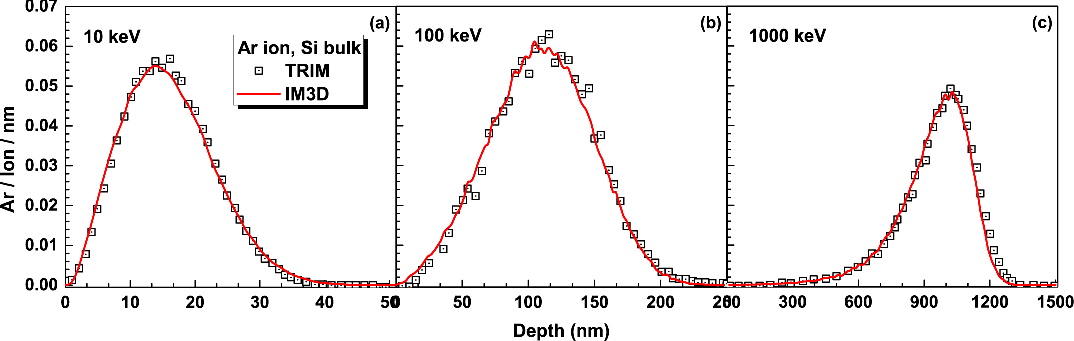
\includegraphics[width=1.0\textwidth]{fig3.pdf}
\caption{Comparison of IM3D results with TRIM predictions for Ar ion depth-distributions in Si bulk, under Ar ion
implantation with different energies of (a) $10~keV$, (b) $100~keV$ and (c) $1000~keV$ and normal incidence at the center point of the target.} \label{Fig.3}
\end{figure}

The vacancy depth-distributions for Ni bulk under He ion beam irradiation with different incident energies are given in Fig.\ref{Fig.4}. Again, good agreements between IM3D and TRIM codes are obtained for all three ion energies. The intensity ratios between the predictions of the FC and KP methods is around 2 as estimated by TRIM code\cite{Stoller:2013}. By comparing to the standard reference values estimated by MD and NRT model, Stoller et al. pointed out that there could be a fundamental problem in the SRIM model used to calculate the number of vacancies created\cite{Stoller:2013}. Borschel et al. also found an obvious discrepancy from Iradina code to TRIM code for the damage production within collision cascades\cite{Borschel:2011}. Since TRIM is not an open-source software, the certain fine details of its defect generation algorithms are not clearly described in both SRIM's manual and published papers\cite{Ziegler:2010}. Generally, this discrepancy should be due to the difference of the replacement fractions in the total displacement events which are determined only by a sharp cut-off threshold energy\cite{Borschel:2011}. This threshold energy is usually set as the displacement energy ($E_d$) as given in SRIM's manual and elsewhere\cite{Ziegler:2010,Borschel:2011}. While the replacement process should occur only when the energy of the trajectory atom after replacement is lower than the binding energy ($E_b$) in bulk. Otherwise, the trajectory atom after replacement will leave the lattice site and migrate to other position, which generate a pair of interstitial and vacancy. Thus, by using the binding energy $E_b$ instead of the displacement energy $E_d$ as the threshold of replacements, we directly reproduced the exact depth profiles with the same absolute values and also the same vacancy intensity ratio between the FC and KP methods. In addition, dynamic annealing process should occur at finite temperatures and the larger number of primary point defects at $0~K$ predicted by the FC method would finally decay to MD, KP or experimental values.
%Thus, it is no need to make much scene to the absolute primary damage concentration at $0~K$ because it is just a reference for practical irradiations at $T>0~K$.

\begin{figure}[!ht]\centering
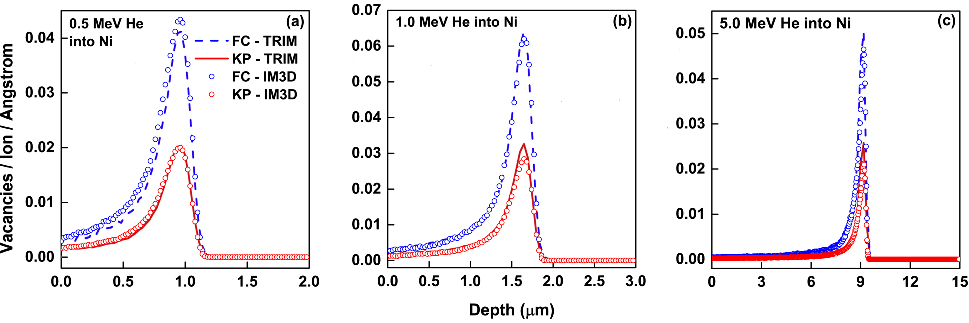
\includegraphics[width=1.0\textwidth]{fig4.pdf}
\caption{Comparison of IM3D results with TRIM predictions for vacancy depth-distributions predicted by FC and KP methods in Ni bulk, under He ion irradiation with different energies of (a) $0.5~MeV$, (b) $1.0~MeV$ and (c) $5.0~MeV$ and normal incidence at the certer point of the target.} \label{Fig.4}
\end{figure}

People found that the range of defect depth-distributions calculated by SRIM package are usually shallower than that of experiments more or less, which generally attributed to an overestimation of the electronic stopping powers used in SRIM package (especially for low-energy heavy ions)\cite{Chang:2012,Zhang:2009,Paul:2013}. A reduced target density is simply employed to compensate for the overestimation of electronic stopping power and thus to reduce the discrepancy\cite{Chang:2012}. Through setting the target density lower, good agreements are obtained comparing to TRIM code and experimental results for $305~nm$ ZrO2 film on Si bulk under $2.0~MeV$ Au ion irradiation, as shown in Fig.\ref{Fig.5}. However, artificially changing of target densities is just a phenomenological treatment with no sound physical basis. Other influences should also be considered to understand this range discrepancy. When ion fluence is high enough, the defect depth-distributions would be physically changed by the evolution of the target density due to ion irradiation. While when ion fluence is not too high, the change of the target density in experiments can be neglected. Moreover, the profiles can further broaden into depth to approach to experiments when taking into account of the diffusion and reaction effects as discussed in our previous paper\cite{Li:2012}. Therefore, it is not only the change of target densities (or the electronic stopping powers) but most of all the diffusion and reaction effects cause the discrepancy, because the temperature in practice is finite other than $T=0~K$ set in TRIM-like codes. The diffusion and reaction effects become prominent especially for the case of ions with much high diffusivity in the target\cite{Li:2012}. These effects are non-equilibrium dynamic processes taking account of temperature and time, which should be described by the meso-scale simulation methods such as the kinetic Monte Carlo (KMC) and cluster dynamics (CD) models.

\begin{figure}[!ht]\centering
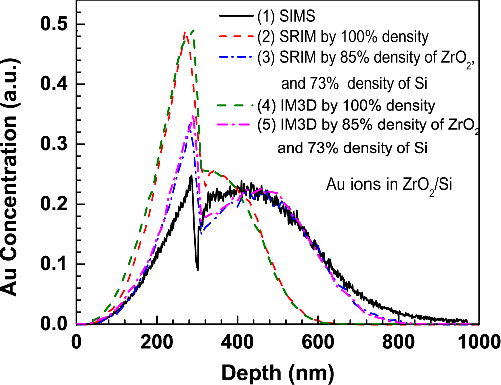
\includegraphics[width=0.6\textwidth]{fig5.pdf}
\caption{Comparison of IM3D results with TRIM predictions and SIMS measurement\cite{Chang:2012} for Au ion depth-distribution in $ZrO_2/Si$ sample, under Au ion irradiation with the energy of $2.0~MeV$ and normal incidence at the center point of the sample. IM3D and TRIM predictions under the assumption of the reduced density are also given, where $15\%$ reduced density for $ZrO_2$ ($4.6~g/cm^3$) and $27\%$reduced density for Si ($1.7~g/cm^3$) are used.} \label{Fig.5}
\end{figure}

%----------------------------------------------------------------------------------------
\section{Two effects: nano-size and geometric effects}

As the ion range or dimension of the collision cascades becomes comparable to the size of the nanoobject itself, the high surface-volume ratio of nanostructured materials will induce two new effects, i.e., the so-called nano-size effect and geometric effect.

Due to the surface reconstruction of nanostructure materials, the thermodynamic properties change with the size reduction, which cause the nano-size effect. In Fig.\ref{Fig.6}(a), the amount of defects along with irradiation energies calculated by IM3D code has the similar trend to that of the analytical model and MD simulation (with the maximum amount produced at energies around $3~keV$), while is smaller than that of MD simulations. This discrepancy should come from the nano-size effects like the difference of stopping powers and the decrease of energy thresholds (i.e., the displacement and binding energies) between nanostrucutres and bulk, etc. While these energy thresholds are usually lower with the size reduction of nanostructures and follow a universal relation as predicted for the cohesive energy of nanoparticles as in Ref.\cite{Vanithakumari:2008}. It would underestimate the total number of defects for both $3$ and $4-nm$ nanowires if the bulk energy thresholds are used for determining the capability of defect generation. This viewpoint can just be proved by using the half values of bulk energy thresholds to decrease the discrepancy between IM3D and MD simulations for the $3-nm$ nanowire. The interstitials, vacancies and sputtering atoms are directly relate to the energy thresholds (especially the surface/lattice binding energies), which are influenced by the nano-size effect mostly. The discrepancy between IM3D and MD simulations thus becomes more obvious when irradiation energy is larger (see Fig.\ref{Fig.6}(b)).

In IM3D code, we consider the bulk parameters are valid at least when the target size is larger than $\sim 10~nm$, because in this case the thermodynamic properties close to constants and the nano-size effect is vanishing\cite{Ouyang:2008}. For the target size smaller than $\sim 10~nm$, IM3D code can also be employed to estimate the primary radiation damages at the first approximation by using a set of modified parameters considered the nano-size effects, while MD method would prefer to be used to give a more accurate estimation because of the acceptable calculation consuming. Furthermore, Fig.\ref{Fig.6} (b) shows that both the nano-size and geometric effects determine the number of defects, that is, the amount of different types of defects for the flat case is higher than that of edge due to the geometric effect. The difference between the flat and edge cases is smaller than that of MD results\cite{Ren:2012}, because no channeling effect is included in IM3D code for an amorphous target.

\begin{figure}[!ht]\centering
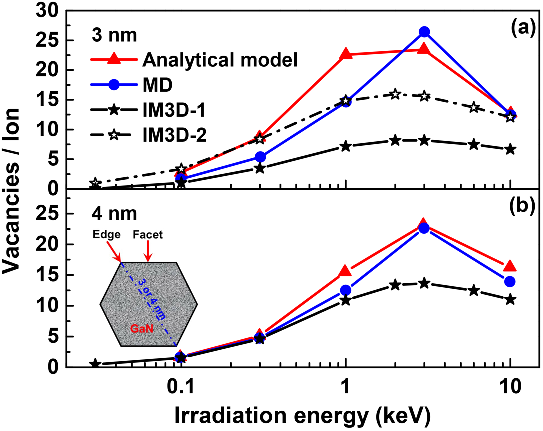
\includegraphics[width=0.49\textwidth]{fig6-a.pdf}
%\label{Fig.1a}
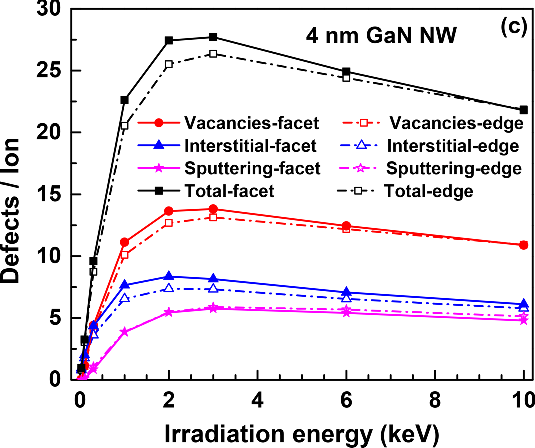
\includegraphics[width=0.46\textwidth]{fig6-b.pdf}
%\label{Fig.1b}
\caption{(a) Comparison of the number of vacancies in GaN nanowire along with Ar ion energies predicted by IM3D code, the analytical model based on TRIM code and MD simulations. The curves for the analytical model are artificially scaled to have the same area as the ones obtained from MD simulations, for the absolute amount of damage cannot be estimated reliably from the results based on SRIM calculations\cite{Ren:2012}. IM3D-1 and IM3D-2 are corresponding to the bulk energy thresholds and half values of the bulk thresholds used in the simulations, respectively. (b) The respect and total numbers for three different types of defects (vacancies, interstitials and sputtered atoms) along with Ar ion energies, for the 3 and $4~nm$-diameter GaN nanowire under Ar ion irradiation at the edge and facet of GaN nanowire.} \label{Fig.6}
\end{figure}

The geometric effect will influence the trajectory of an ion when it transport through the interface between two different material zones, such as trajectory emission, re-entering, sputtering and shading, etc. In order to illustrate the geometric effect contrast to the bulk counterpart, we simulate the vacancy depth-distributions in Au column target under two types of ion beams (i.e. center and random incidence), as shown in Fig.\ref{Fig.7}. The ranges of vacancy depth-distributions and the total amount of vacancies are both increase with the increasing of column diameters, and finally approach to the bulk values after the critical diameters (around $200~nm$ and $1000~nm$ for center and random ion incidence, respectively).

Assumes that the radial distribution of damages (e.g. vacancies) $I \left( r \right)$ produced by an ion in a half-infinite bulk target follows a exponential decay (as shown by the inserted figure in Fig.\ref{Fig.7}(a)),

\noindent
\begin{equation}
I\left(r\right) = I_0 e^{-r/t},~~r \in \left[0, \infty\right), \label{Eq.1}
\end{equation}

\noindent where, $I_0$ is the intensity of damages at $r=0$ and $t$ is the effective attenuation length of damages in radial direction ($25~nm$ for center ion incidence). The amount of damages in a nanowire for the center ion beam incidence can be obtained by integrating Eq.(\ref{Eq.1}) over the volume of the antisymmetric column (see Fig.\ref{Fig.7}) that,

\begin{equation}
N_d = \int_{0}^{R} \int_{0}^{2\pi} I\left(r\right)drd\theta = \frac{2 \pi I_0}{t} \left(1-e^{-R/t}\right), \label{Eq.2}
\end{equation}

\noindent where R is the radius of the column.

Similarly, we can give the analytical function for the random ion beam incidence, by additionally considering the effective attenuation range $t$ ($32~nm$ for random ion incidence) of the spread ion beam. For $R \leq t$, we assumed that the amount of damages also follows Eq.(\ref{Eq.2}) approximately but with $t=32~nm$ instead. While for $R > t$, only ions bombarding in the effective attenuation range $t$ from the colume side with the area ratio of $\left( \frac{2t}{R} - \frac{t^2}{R^2} \right)$, can cause a half loss of defects with the ratio of $0.5 \cdot \left(1 - \frac{1}{e}\right)$ as estimated approximately from Eq.(\ref{Eq.2}) with $R = t$. Otherwise, no loss of the defects when ions bombarding in the central zone $(0,~R-t)$ of the column. Thus, the amount of damages follows that,

\begin{equation}
N_d = \frac{2 \pi I_0}{t} \left[1 - 0.5 \cdot \left( \frac{2t}{R} - \frac{t^2}{R^2} \right) \left(1 - \frac{1}{e}\right) \right],~ R > t. \label{Eq.3}
\end{equation}

\noindent It can be found as shown in Fig.\ref{Fig.7} that these two simple analytical estimations can fit the calculated vacancy-diameter relation much well, which directly illustrates that the geometric effect is the main factor to the distributions of primary radiation damages in nanostructured materials.

\begin{figure}[!ht]\centering
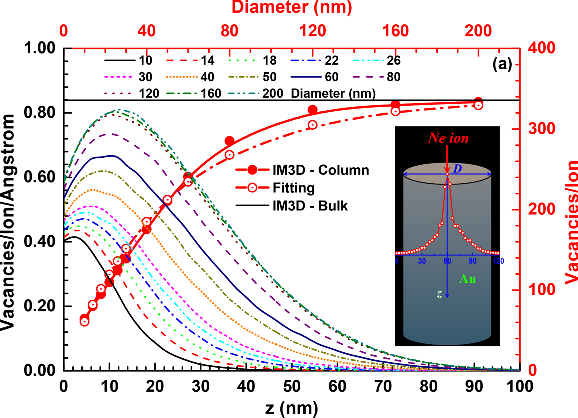
\includegraphics[width=0.49\textwidth]{fig7-a.pdf}
%\label{Fig.1a}
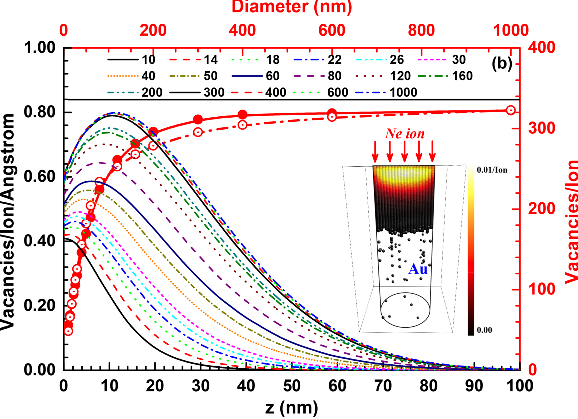
\includegraphics[width=0.49\textwidth]{fig7-b.pdf}
%\label{Fig.1b}
\caption{The depth-distributions and the total number of vacancies for Au nanowaire with different diameters under $45~keV$ Ne ion irradiation with the (a) center and (b) random normal-incidence beams. Eqs.(\ref{Eq.2}) and (\ref{Eq.3}) are plotted to fit the relations of the total number of vacancies with different diameters. The inserted figures in (a) and (b) show the vacancy radial-distribution in Au bulk and the vacancy space-distribution in Au nanowire with the diameter of $120~nm$, respectively.} \label{Fig.7}
\end{figure}

Column is a typical model of a class of nanostructured materials, such as nanowire, nanoporous and ``fuzz''. Bringa et al. performed a serial of experimental studies on the anti-irradiation behaviors of nanoporous materials and proposed an anti-irradiation window by simply considering of the effective vacancy diffusivity and lower critical size due to melting. However, they did not consider the contribution from the change of primary radiation damages by the geometric effect and just assumed that the primary radiation damages is a constant value. As shown here, the geometric effect can introduce a dramatical reduction of the primary radiation damages, which should be taken into account in the estimation of the anti-irradiation window. Furthermore, by considering the primary damage distributions as well as the diffusion and reaction effects at $T > 0~K$, CD model would be performed to give the more accurate anti-irradiation windows of nanostructure materials in the future.

%----------------------------------------------------------------------------------------
\section{Applications}

\subsection{Arbitrary complex targets based on CSG and FETM methods}

To our knowledge, IM3D is the most universal and robust code for simulating of the primary radiation damages in arbitrary complex targets with different shapes and components till now. Based on CSG geometric model, nine basic shapes (in Fig.\ref{Fig.8}(a)) and their assemblies (in Fig.\ref{Fig.8}(b)) can be constructed at present to model many regular targets with different materials. The geometric effect makes the distinctions of the defect space-distributions among different shapes.

\begin{figure}[!ht]\centering
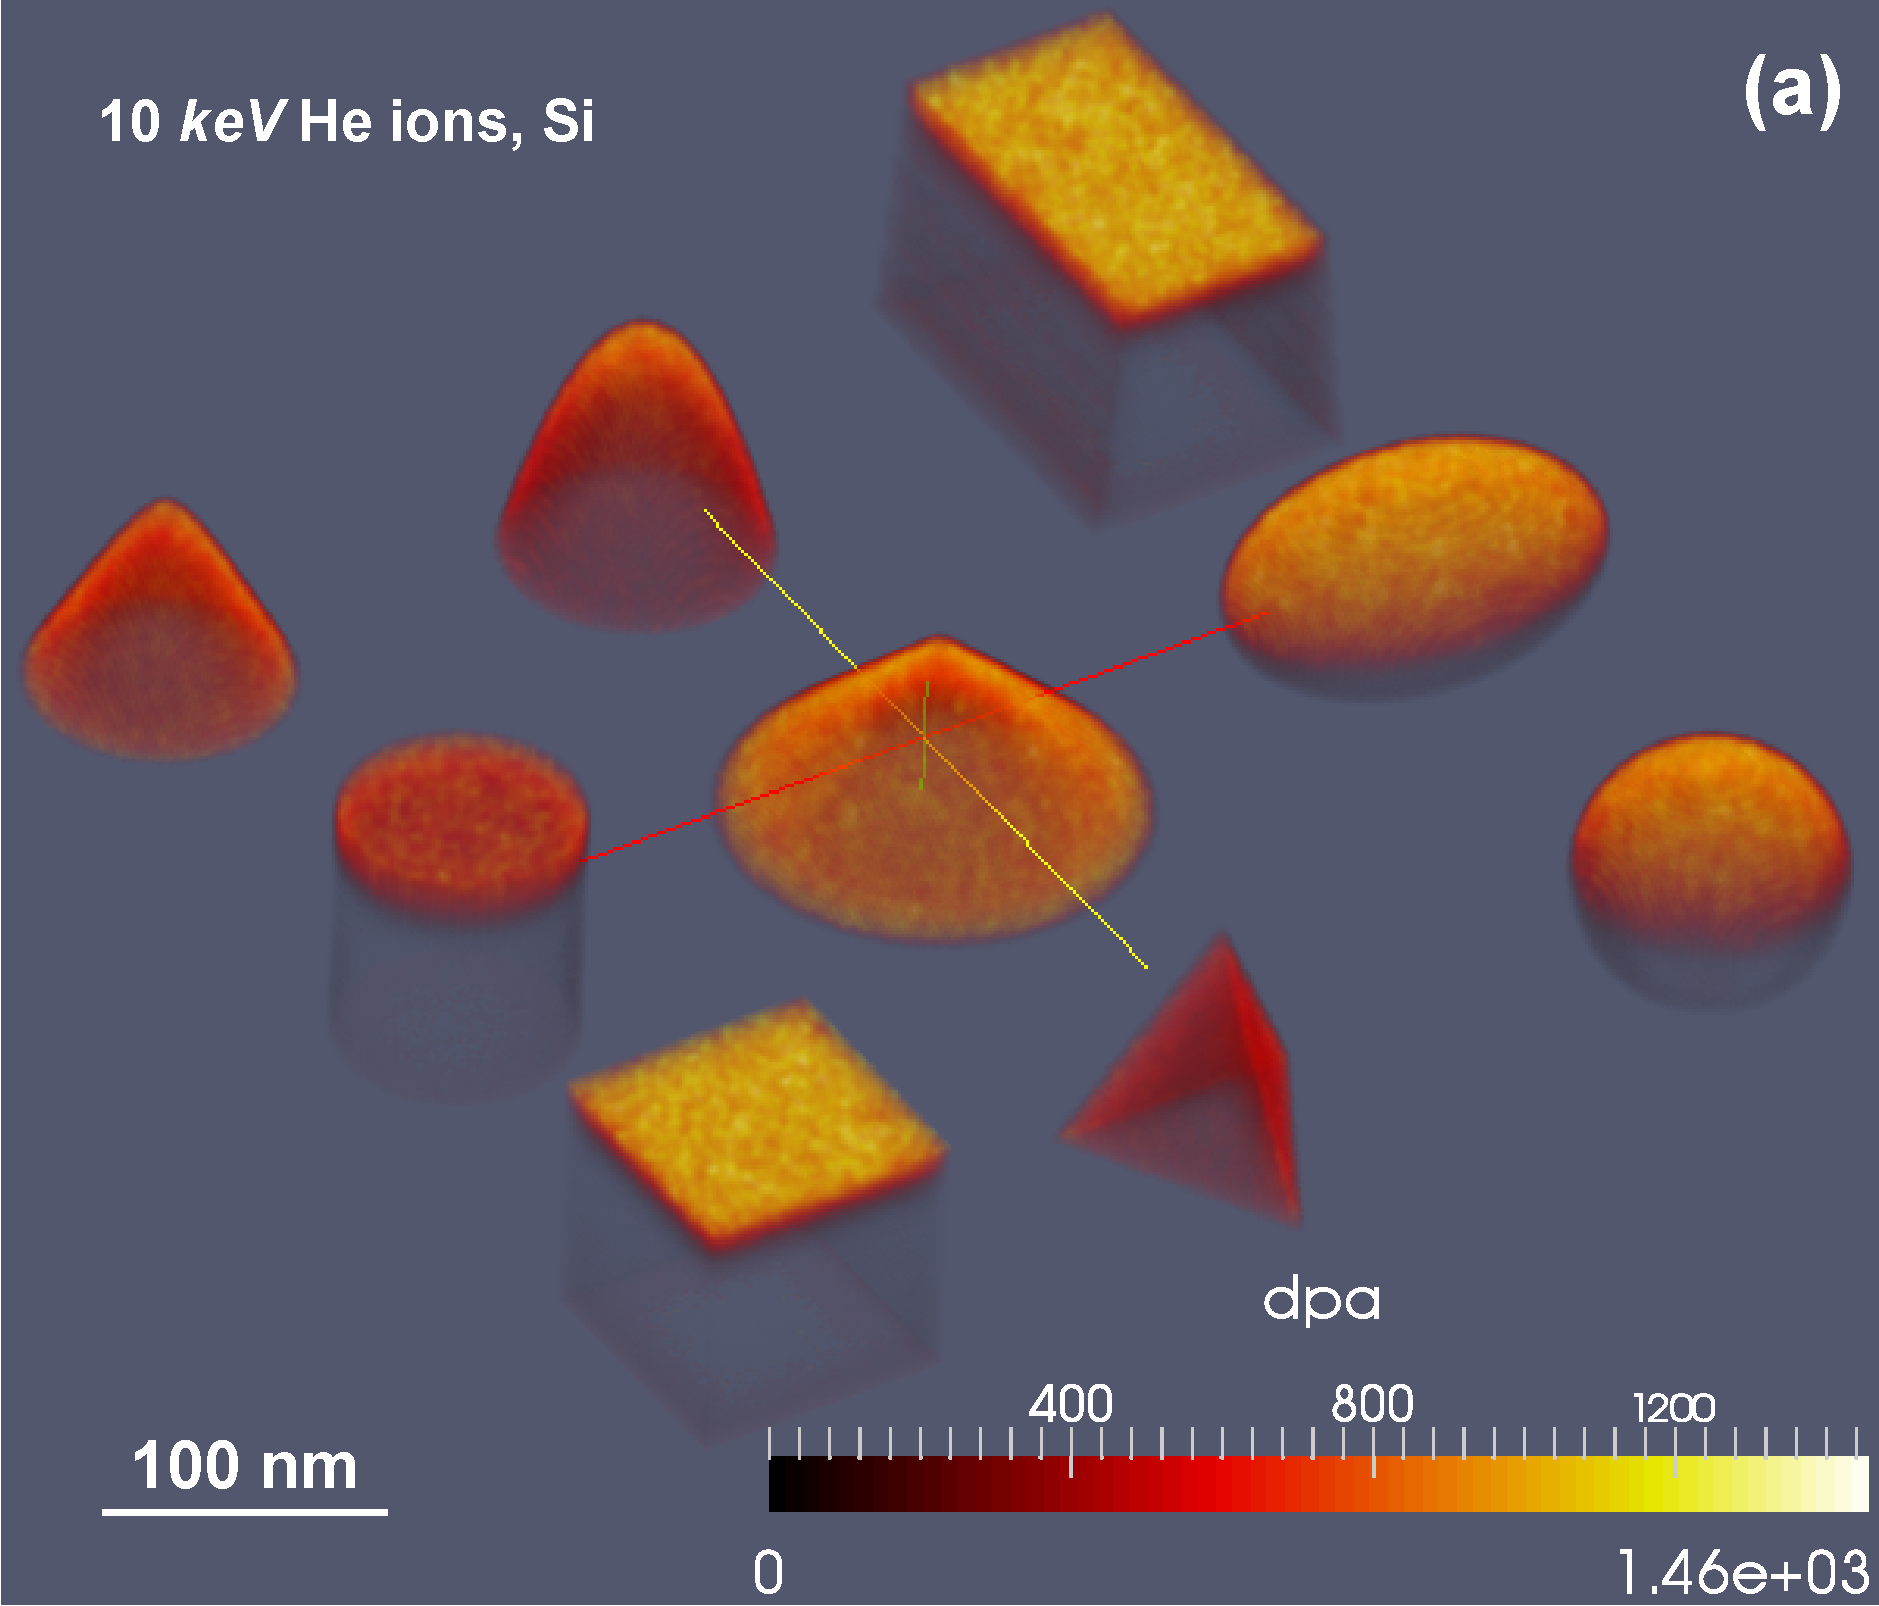
\includegraphics[width=0.32\textwidth]{fig8-a.pdf}
%\label{Fig.1a}
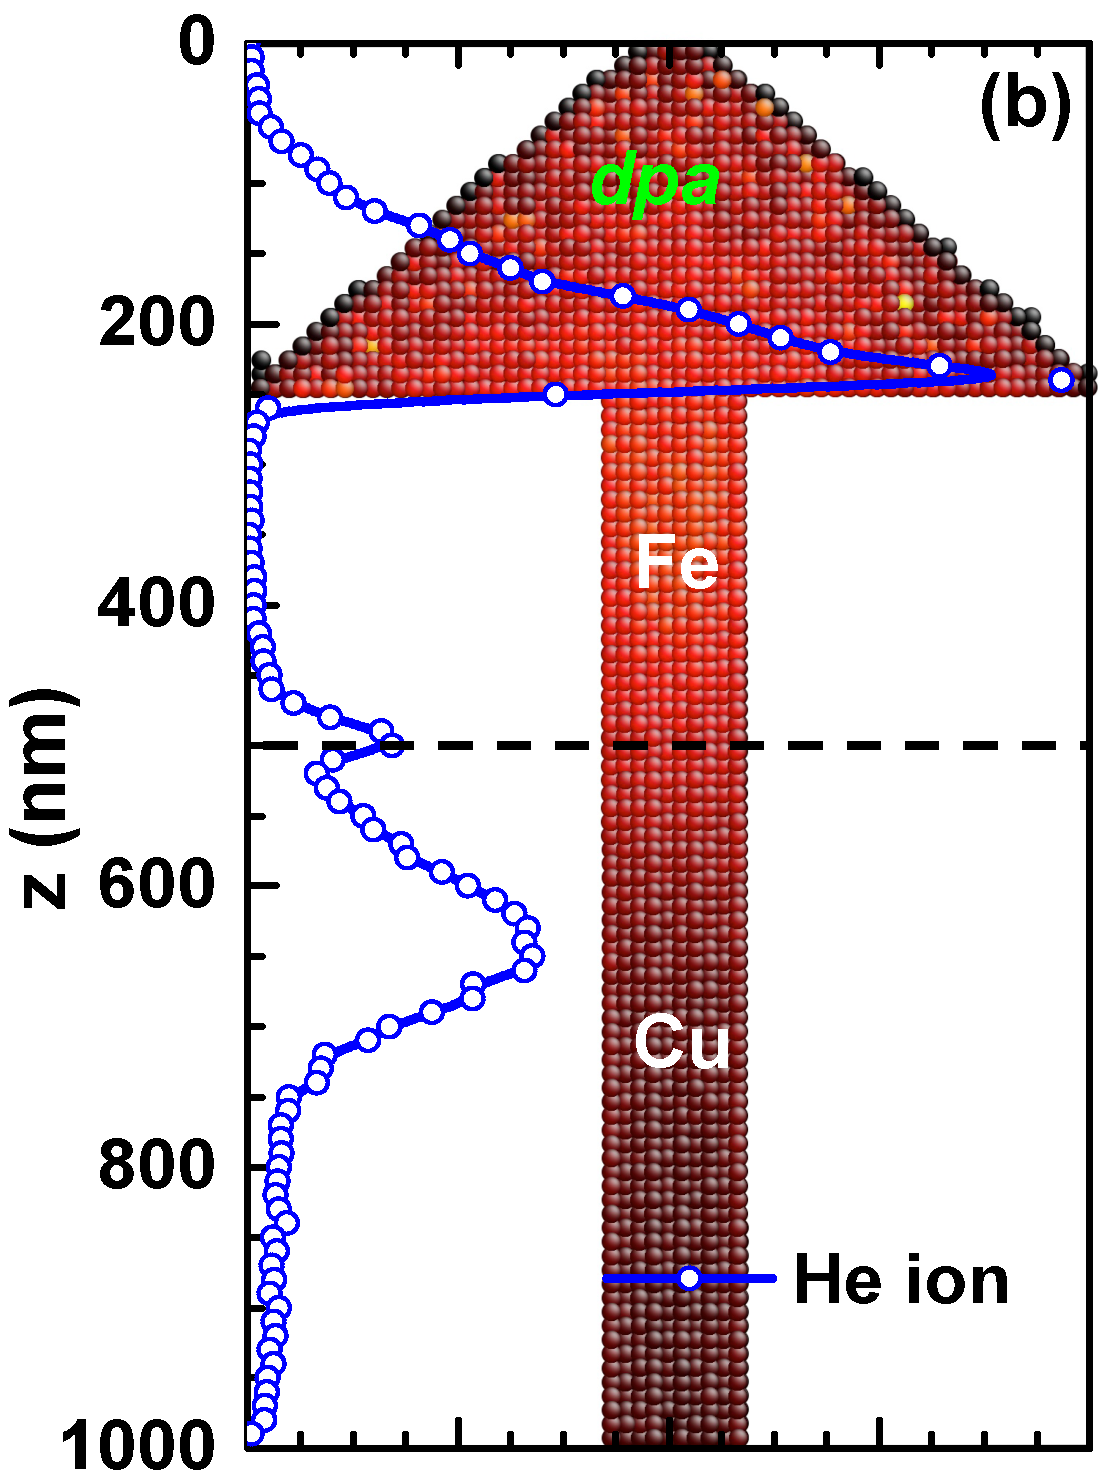
\includegraphics[width=0.21\textwidth]{fig8-b.pdf}
%\label{Fig.1b}
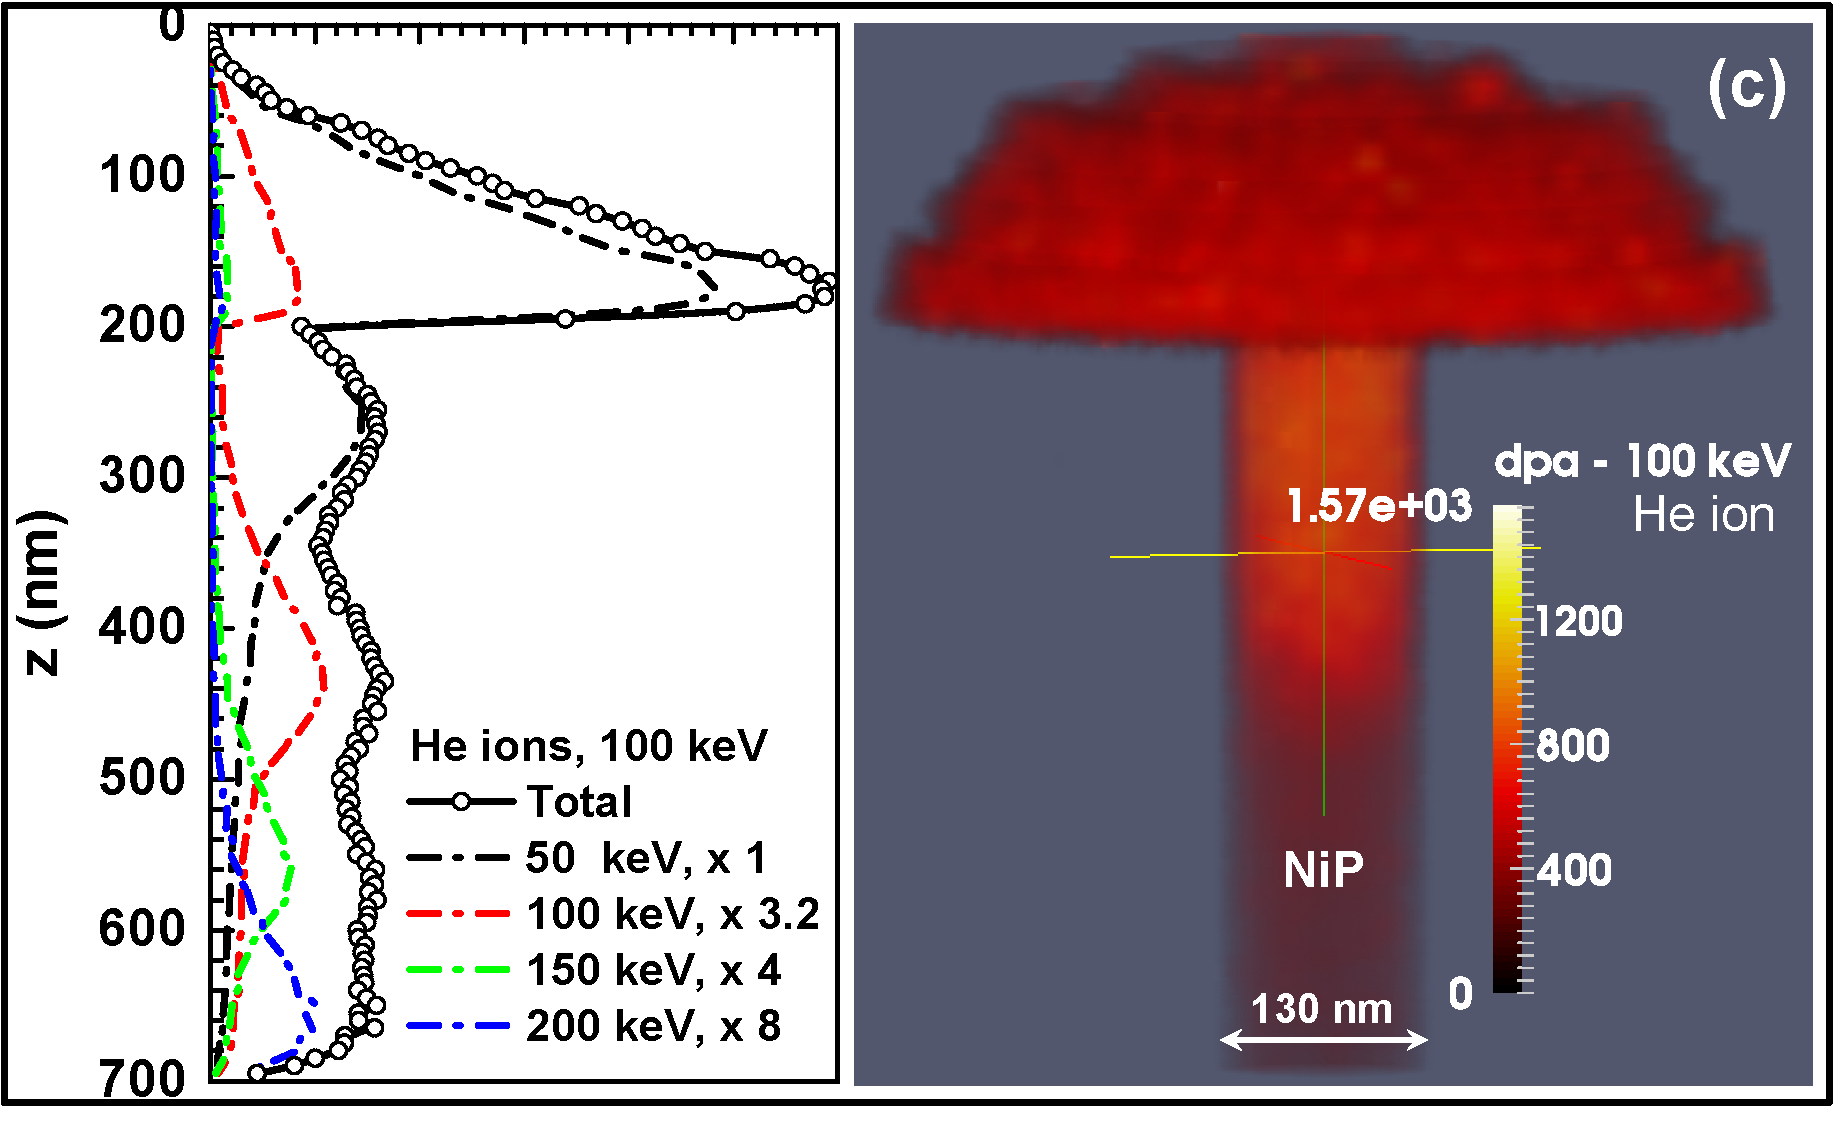
\includegraphics[width=0.44\textwidth]{fig8-c.pdf}
%\label{Fig.1b}
\caption{(a) $Dpa$ space-distributions of nine basic shapes based on CSG geometric method and composed of Si under $10~keV$ He ion irradiation with the random normal-incidence beam. (b) $Dpa$ space-distribution of for a 100 nm-diameter Cu/Fe nano-bicrystal constructed by CSG geometric method under $200~keV$ He ion irradiation with the random normal-incidence beam. The insert scatter line is the corresponding He ion depth-distribution. (c) The respect and total He ion depth-distributions for different energies He ions (left) and the $dpa$ (right) space-distribution for $100~keV$ He ions with the random normal-incidence beam irradiated on a $130~nm$ NiP metallic glass nanostructure constructed by FETM geometric method.} \label{Fig.8}
\end{figure}

By introducing the geometric effect, more reliable information can be obtained when estimate the defect (such as ion and $dpa$) distributions. For bulk/multi-layer systems, people usually employ TRIM code to give the first approximation of ion/dpa distributions. However, for complex nanostructures as mentioned in Refs.\cite{Liontas:2014,Landau:2014}, errors would be introduced when using TRIM code. As shown in Fig.\ref{Fig.8}(b), more practical $dpa$ space-distribution is obtained for a Cu/Fe nano-bicrystal based on CSG geometric model. For NiP metallic glass nanostructures (in Fig.\ref{Fig.8}(c)), more accurate ratio of ion fluence can be estimated to generate a uniform distribution damage based on FETM geometric model, with $1:3.2:4:8$ instead of $3.5:4.0:2.8:5.5$ in Ref.\cite{Liontas:2014}. Thus, the geometric effect can dramatically change the behaviors of ion irradiation and can not be neglected.

\subsection{Nano-yttria in ODS steels under ion-irradiation}

Recently, ODS steels (with a great mount of yttria ($Y_2O_3$) nanopartiles embedded in a steel matrix) have been termed as a new class of high anti-irradiation and high strength nanostructured nuclear materials\cite{Chen:2013,Brimbal:2014,Fave:2014,Huang:2014,Lazauskas:2013,Lescoat:2012}. However, the high radiation resistant mechanisms and the role of the embedded nanoparticles are still unclear and sometimes controversial. Moreover, the impact of primary damage processes on their high radiation resistant properties should also be discussed in detail. Here, we assumes a perfect iron matrix in which $Y_2O_3$ nanoparticles are embedded as a simplified model of an ODS steel and simulate the space-distributions of the primary radiation damages with the displacement energies of $40~eV$\cite{Ziegler:2010} for Fe and $57~eV$ for Y and O\cite{Lescoat:2012}.

\begin{figure}[!ht]\centering
\includegraphics[width=0.5\textwidth]{fig9.pdf}
\caption{The (a) ion trajectories and (b) $dpa$ distribution cross-section for a target of Fe matrix with a void ($30~nm$) and two $Y_2O_3$ nanoparticles ($30~nm$ and $10~nm$) of different sizes embedded under $150~keV$ Fe ion irradiation with the random normal-incidence beam.} \label{Fig.9}
\end{figure}

Based on IM3D code, the ion trajectories and 3D space-distributions in a target of Fe matrix with a void and two $Y_2O_3$ nanoparticles of different sizes embedded can be given as shown in Fig.\ref{Fig.9}. Spheres with different materials/vacuum can change ion trajectories (Fig.\ref{Fig.9}(a)) by influencing the energy losses and the production rate of defects, and finally induce the different damage distributions (in Fig.\ref{Fig.9}(b)). Comparing to bulk regions, ions in void transport straightly without energy loss and penetrate into depths to generate more damages in the deep (i.e., the enhancement effect, similar to the MD results\ref{Lazauskas:2013}). Similarly, ions can also loss less energy and generate less damages in $Y_2O_3$ nanoparticles. Thus, $Y_2O_3$ nanoparticles are play the same role as voids to suppress the production of primary radiation damages but without losing the strength of the steel. The anti-irradiation of $Y_2O_3$ nanoparticles is mainly due to the lower defect generation rate with their much lower atomic density ($1.10934 \times 10^{22}~atoms~cm^{-3}$) comparing to that of the steel matrix ($8.388 \times 10^{22}~atoms~cm^{-3}$), the higher displacement energies of Y and O ($57~eV$) to that of Fe ($40~eV$), as well as the attraction of defects to the nanoparticle interface during annealing. The enhancement effect of $dpa$ intensity behind the void and  the bigger-size $Y_2O_3$ nanoparticle comes from the overlapping of the $dpa$ generated by the penetrating ion though the void / nano-particle and the ion directly transporting in iron matrix nearby, as shown in Fig.\ref{Fig.9}(a). This enhancement effect would induce a little more serious primary damages to Fe bulk matrix, which introduce a negative effect on the radiation resistant. While the enhancement effect can be reduced/removed by decreasing the diameter of $Y_2O_3$ nanoparticles from $30~nm$ to $10~nm$ as shown in Fig.\ref{Fig.9}(b), which has also been proved by the high resolution TEM measurements\cite{Lescoat:2012}. The high sink strength of the interface between $Y_2O_3$ nanoparticles and Fe matrix would also neutralize the enhancement effect and finally reduce the total damages in ODS steel after annealing.

\subsection{Ion beam sputtering induced the bending of W nanowire}

Under ion beam irradiation with high fluence, nanowires have been observed to bend towards and finally align with the ion beam\cite{Cui:2013}. The primary radiation damages should play an important role on this effect, which can also be studied by IM3D code feasibly. By generating a target with 3D surface mesh with FETM geometric method beforehand (in Fig.\ref{Fig.10}(a)) and inputting it into IM3D code, the 3D distribution of defects can be given such as vacancies for a bended W nanowire under the irradiation of Ga ion with the incident direction of 40 degrees and the energy of $150~keV$, as shown in Fig.\ref{Fig.10}(b). More primary vacancies generated on the side towards to the ion beam, making the density on this side lower than the other side and thus bend the column line. During the ion irradiation of W nanowire at finite temperatures, most of interstitials with a low migration energy ($0.013~eV$\cite{Derlet:2007}) would anneal with vacancies immediately, diffuse to the other side or deposit directly. While a little part of vacancies without annealing by interstitials are nearly immobile and stay constant with a much higher migration energy ($1.66~eV$\cite{Becquart:2007}). Here, in order to consider the final remaining damages in W nanowire, we use the difference value of vacancies minus interstitials by assuming annihilation of defects only occur in each cell ($10 \times 10 \times 10~nm^3$). An inhomogeneous distribution of the remaining defects is given in Fig.\ref{Fig.10}(c), where excess vacancies remain on the side towards to the ion beam and excess interstitials remain at the opposite side. Thus, a bending momentum (under inner stress due to an inhomogeneous expansion of the nanowire) towards the ion beam is induced to compensate the density difference until the the direction of the column line along the direction of ion beam, as observed in the experiment\cite{Cui:2013}. Moreover, the shading/shadowing effect (shading of the ions on their incident path by a particle leads to a decrease of damages behind the particle) can also be seen in Fig.\ref{Fig.10}(b) with dark area in the substrate appear behind the nanowire. During the plasma-surface interaction (PSI) process in PFMs (as shown below), these two typical effects (i.e., the bending and shading effects) should also occur at the reconstructed surface, causing the formation of complex ``fuzz'' nanostructure finally.

\begin{figure}[!ht]\centering
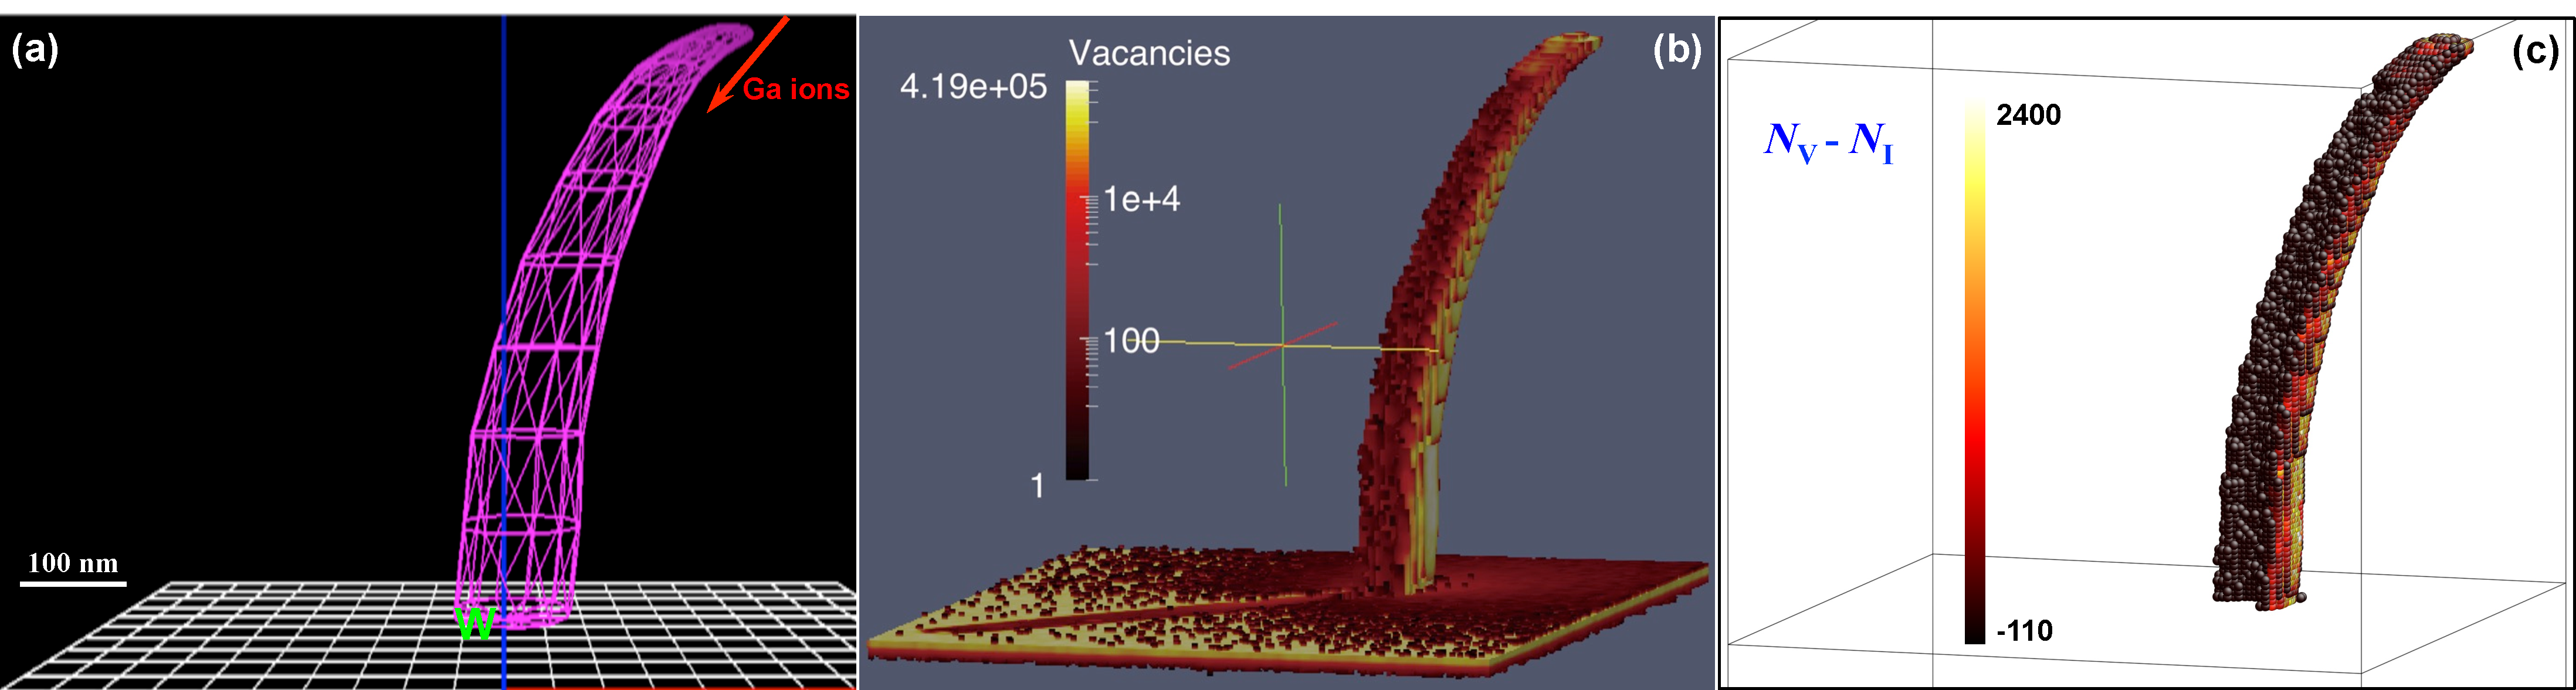
\includegraphics[width=1.0\textwidth]{fig10.pdf}
\caption{The (a) 3D surface mesh with FETM geometric method, (b) vacancy space-distribution and (c) remaining excess vacancies for a bended W nanowire under randomly distributed Ga ion sputtering with the incident direction of 40 degrees and the energy of $150~keV$.} \label{Fig.10}
\end{figure}

\subsection{D retention in W with roughness surface}

Plasma-surface interaction (PSI) is one of the most important issue in nuclear fusion instruments. Under low energy (in the range of $10 - 100~eV$), high flux (up to the order of $10^{24}~m^{-2}s^{-1}$) D/T/He plasma loads in ITER\cite{Wirth:2014}, the near surface morphology of PFMs will be dramatically changed and reconstructed to roughness or even more complex nanostructures like ``fuzz". These roughness nanostrucutes would further increase the retention of D/T/He. While T retention is also another key problem need to be widely studied. Thus, the calculation of the primary retention of H isotopes in W with roughness structures is much helpful for the understanding of the mechanisms of surface damage and T retention in PFMs.

In Fig.\ref{Fig.11}, we performed the W bulk with different rough-surface under D ion irradiation. A simple geometric model based on FETM method are used here to simulate the roughness structures\cite{Li:2008}. The rough-surface is constructed in a finite element triangulated mesh by using a Gaussian function to describe the distribution of the amplitude ($3 \sigma$) of the random roughness peaks as well as a uniform square mesh with a lattice constant ($a = 50 ~nm$) to describe the density of the roughness peaks. The depth-distributions of D in W are given for different rough amplitudes ($3 \sigma$) from $9$ to $1000~nm$ (in Fig.\ref{Fig.11}(b)). We found that the range of D ions in W increase with the increasing of rough amplitude. The distributions relate to Gaussian distribution directly, which can be approximated by the convolution of the effective interaction range and the geometric distribution of rough-surface, as shown in Fig.\ref{Fig.11}(b). Also, the geometric and shading effects dominate the behavior of D retention in W bulk with roughness surface.

The relation of D retention rate with the rough amplitude is also given in Fig.\ref{Fig.11}(c). With the increasing of the rough amplitude, D retention rate decreases at first and then increase after a critical point at about $3 \sigma = 50~nm$. It should be due to the competition of the enhancements of both the backscattering at glancing incidence and the shading effect by rough peaks. In order to describe the exact relation of the retention rate with the geometric and shading effects, a simple model is introduced to fit this relation. For the amplitude and distance of the roughness peaks are set as $3 \sigma$ and $a$, the effective incident angle of ions related to rough-surface is $\alpha \doteq arccos \left( \frac{a}{\sqrt{\left(3 \sigma \right)^2 + \left( a \right)^2}} \right)$. The backscattering coefficient $\eta \left(\alpha \right)$ is the function of this effective incident angle $\alpha$, which can be calculated by IM3D code directly. Thus, for the zero-order approximation, the primary retention rate of ions is equal to,

\noindent
\begin{equation}
R_0 \left( \alpha \right) \doteq 1 - \eta \left(\alpha \right), ~~all~3 \sigma. \label{Eq.4}
\end{equation}

\noindent Here, we assumed that it is actually true when $3 \sigma \leq z_0$, where $z_0 = 50~nm$ is used. While for $3 \sigma > z_0$, a fraction of backscattered ions would be shaded and redeposited by the roughness peaks, the shading probability can be estimated by the geometric effect as $P_s = \int_{0}^{\alpha} sin \left( \theta \right) d \theta = 1 - cos \alpha$. Thus, by assuming that all of the shaded ion are redeposited by the roughness peaks for the first-order approximation, the primary retention rate of ions can be described by,

\noindent
\begin{equation}
R_1 \left( \alpha \right) \doteq \left( 1 - \eta \left( \alpha \right) \right) + \eta \left( \alpha \right) \left( 1 - cos \alpha \right) = 1 - \eta \left( \alpha \right) cos \alpha, ~~ 3 \sigma > z_0. \label{Eq.5}
\end{equation}

\noindent If considering there is still some probability ($R_1$ is approximately used here) for the escaping of the shaded ions by roughness peaks, a more accurate estimation of the primary retention rate of ions in rough-surface can be given by a second-order approximation base on the predictor-corrector method,

\noindent
\begin{eqnarray}
& R_2 \left( \alpha \right) & \doteq \left( 1 - \eta \left( \alpha \right) \right) + R_1 \left( \alpha \right) \eta \left( \alpha \right) \left( 1 - cos \alpha \right) \nonumber \\
&&{} = 1 - \eta \left( \alpha \right) cos \alpha - \eta ^2 \left( \alpha \right) cos \alpha + \eta^2 \left( \alpha \right) cos^2 \alpha, ~~ 3 \sigma > z_0. \label{Eq.6}
\end{eqnarray}

\begin{figure}[!ht]\centering
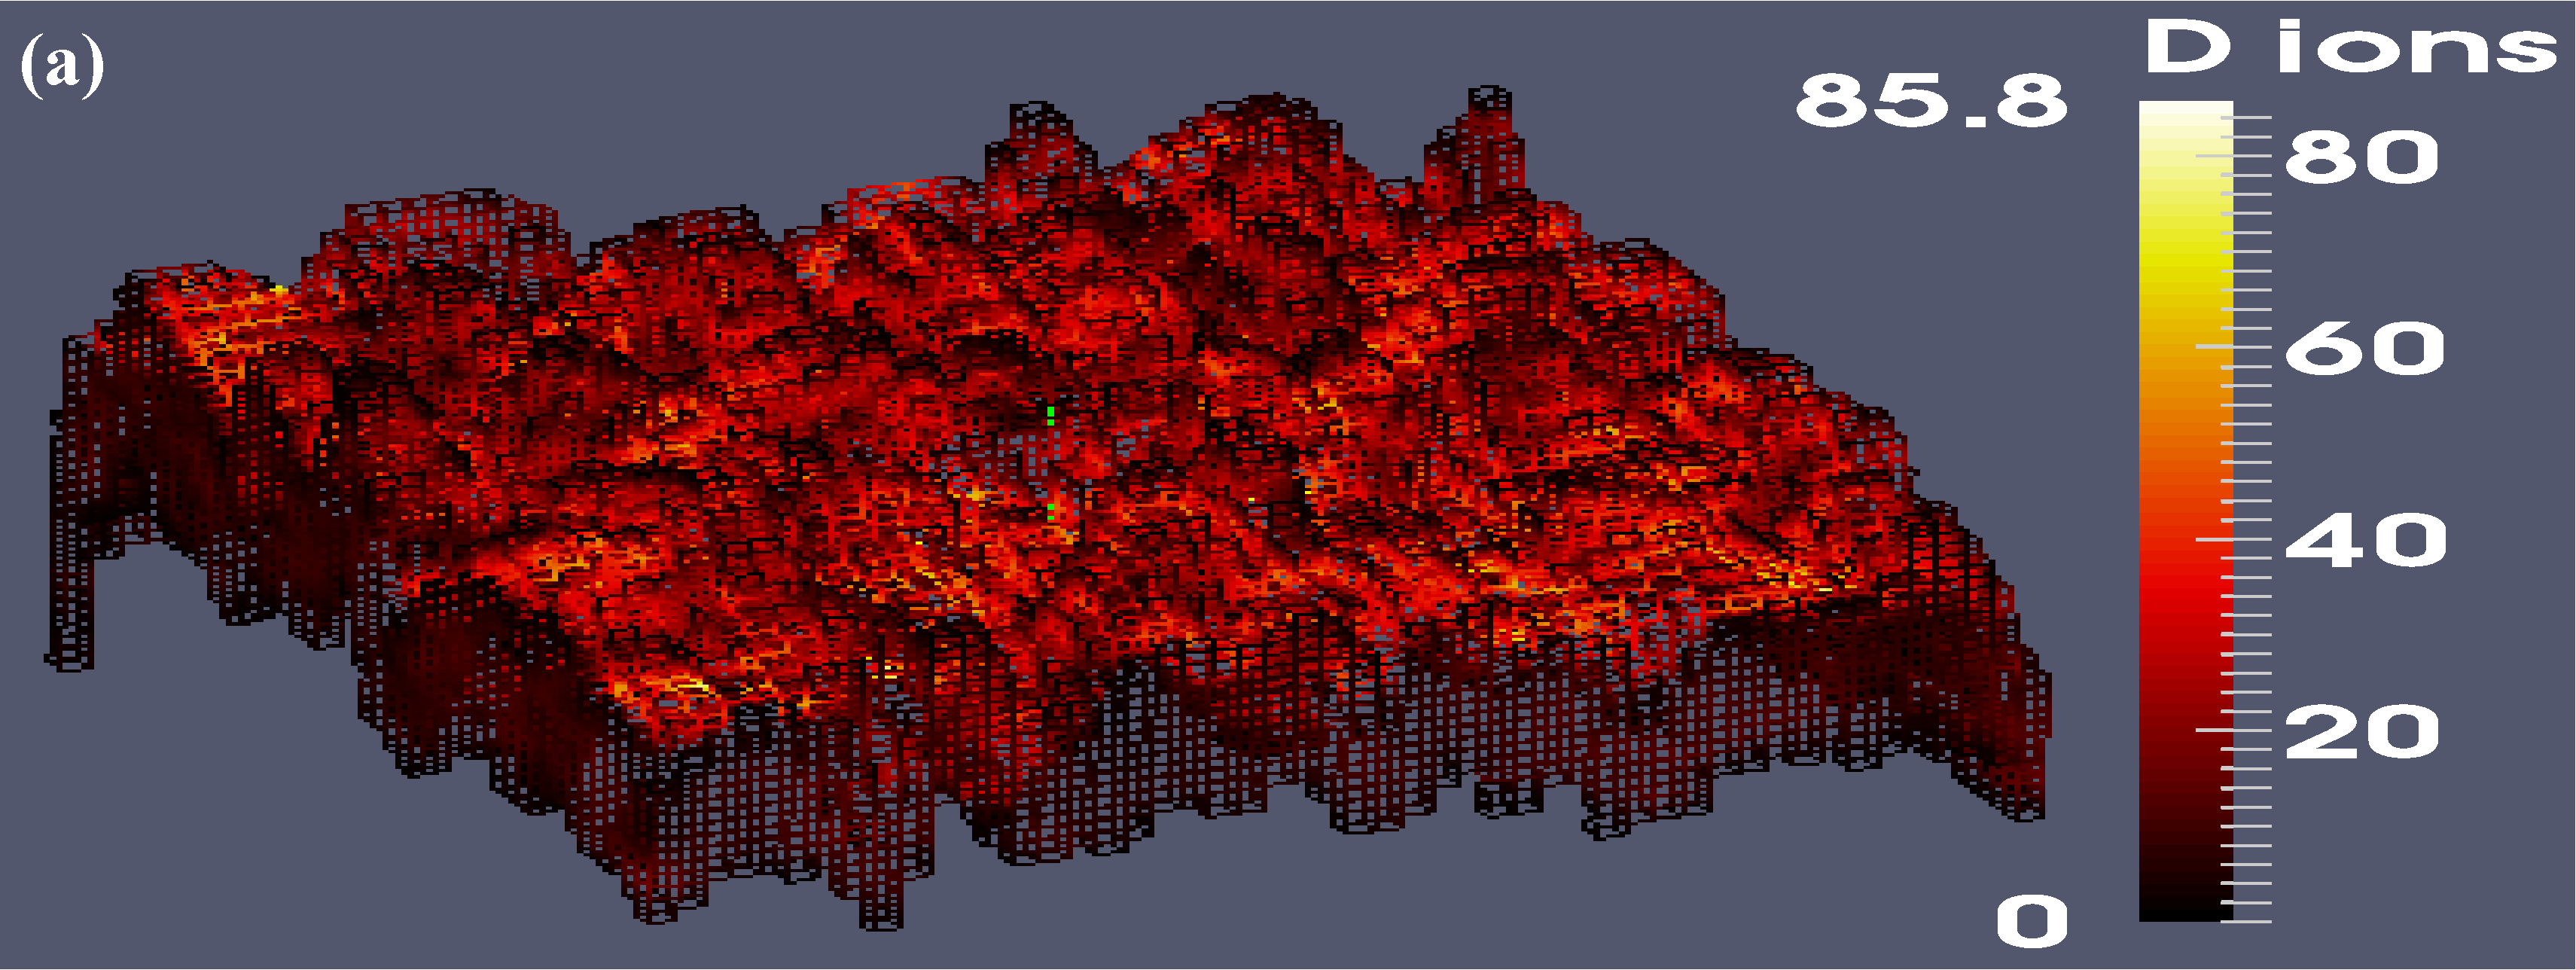
\includegraphics[width=0.65\textwidth]{fig11-a.pdf}
%\label{Fig.1a}
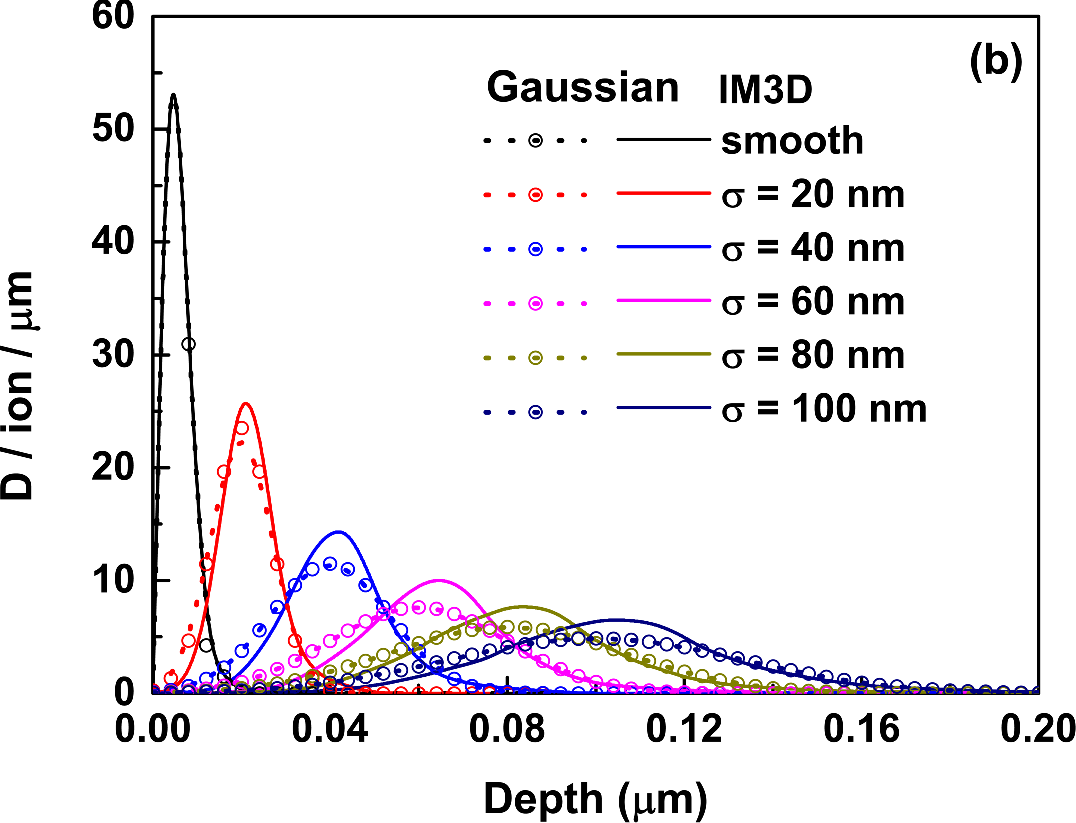
\includegraphics[width=0.51\textwidth]{fig11-b.pdf}
%\label{Fig.1b}
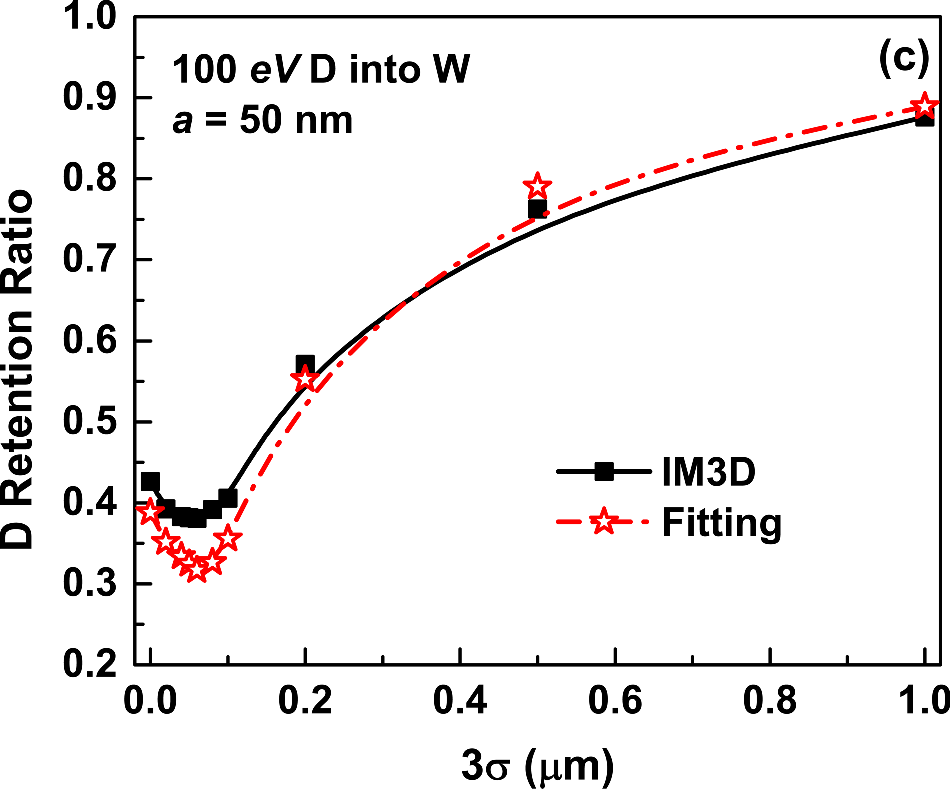
\includegraphics[width=0.47\textwidth]{fig11-c.pdf}
%\label{Fig.1c}
\caption{(a) The D ion space-distribution for W roughness surface with the roughness amplitude of $3 \sigma = 60~nm$ and the roughness constant of $a = 50~nm$. (b) The D ion depth-distributions and the fitting profiles by Gaussian functions for W roughness surface with different roughness amplitudes ($3 \sigma$) and the roughness constant of $a = 50~nm$. (c) The D retention ratio and the fitting Eqs.(\ref{Eq.4}) and (\ref{Eq.6}) along with the roughness amplitudes for W roughness surface with the roughness constant of $50~nm$. Here, all W roughness surfaces are under the irradiation of $100~eV$ D ion beam with the random normal-incidence.} \label{Fig.11}
\end{figure}

A good agreement can be given based on the rough estimations by Eq.(\ref{Eq.4}) for $3 \sigma \leq z_0$ and Eq.(\ref{Eq.6}) for $3 \sigma > z_0$ (as shown in Fig.\ref{Fig.11}(c)), which demonstrates that the geometric and shading effects are the main contributions to the enhancement of the primary D retention in W. At finite temperature or especially high temperatures (typically $400 - 800~^\circ C$ in ITER\cite{Wirth:2014}) in fusion instruments, interstitial D atoms will diffusion quickly, most of which would desorb from surface. While, if the influence of the diffusion effect is fixed, the primary retention rate would be the only key factor to the D retention, especially when the surface of PFMs becomes roughness. Furthermore, the retention of D/T/He in ``fuzz" structures should also follow the same trend at a first glance.

% Chapter 7

\chapter{Additional Tools}  % Main chapter title

\label{Chapter7}  % For referencing the chapter elsewhere, use \ref{Chapter1}

\lhead{Chapter 7. \emph{Additional Tools}}  % This is for the header on each page - perhaps a shortened title

%----------------------------------------------------------------------------------------

\section{Config.in file generation code}

gen\_config\_in

%----------------------------------------------------------------------------------------

\section{Shape files generation code}

gen\_shape

\subsection{CSG}


\subsection{FETM}

%----------------------------------------------------------------------------------------

\section{}

%----------------------------------------------------------------------------------------


% Chapter 8

\chapter{Errors and Warnings}  % Main chapter title

\label{Chapter8}  % For referencing the chapter elsewhere, use \ref{Chapter1}

\lhead{Chapter 8. \emph{Errors and Warnings}}  % This is for the header on each page - perhaps a shortened title

%----------------------------------------------------------------------------------------

\section{}


%----------------------------------------------------------------------------------------

\section{}


\subsection{}


\subsection{}


\subsection{}


%----------------------------------------------------------------------------------------

\section{}


\subsection{}


%----------------------------------------------------------------------------------------

\section{}

\subsection{}


\subsection{}


%----------------------------------------------------------------------------------------

\section{}


%----------------------------------------------------------------------------------------

\section{}

%----------------------------------------------------------------------------------------



%----------------------------------------------------------------------------------------
%	THESIS CONTENT - APPENDICES
%----------------------------------------------------------------------------------------

\addtocontents{toc}{\vspace{2em}} % Add a gap in the Contents, for aesthetics

\appendix % Cue to tell LaTeX that the following 'chapters' are Appendices

% Include the appendices of the thesis as separate files from the Appendices folder
% Uncomment the lines as you write the Appendices

% Appendix A

\chapter{Physical models} % Main appendix title

\label{AppendixA} % For referencing this appendix elsewhere, use \ref{AppendixA}

\lhead{Appendix A. \emph{Physical models}} % This is for the header on each page - perhaps a shortened title

In IM3D code, the simulation of ion transportation in matter proceeds is similar to the well-established TRIM-like codes, which basically introduces the random phase approximation (RPA), the binary collision approximation (BCA) and the central potential approximation (CPA)\cite{Ziegler:2010,Schiettekatte:2008,Biersack:1980}. The code simulates numerical random trajectory histories of ions to present statistically meaningful calculation results. Each trajectory corresponds to a particle (ion or target atom) with a specified starting position, a given direction and an incident energy. The particle is tracked as a random sequence of straight free-flight-paths that end with a binary nuclear collision event where the particle changes its direction of movement and/or reduces energy as a result of nuclear (elastic collision process) and electronic (inelastic collision process) energy losses. The energy and direction of the particle from incident direction are thus updated from the conservation of energy and momentum. Where, the probability of energy losses depends on the target atom density, as well as the nuclear and electronic stopping powers which can be assumed to be independent. Meanwhile, point defects could be produced in elastic collision events. Finally, the trajectory is terminated till the energy of the particle drops below a specified value $E_{min}$ or the particle leaves the target. A program chart of the ions tracing and defects generation in a target is given in Fig.\ref{Fig.1} and the detailed physical background can also be found elsewhere\cite{Ziegler:2010}.

\begin{figure}[!ht]\centering
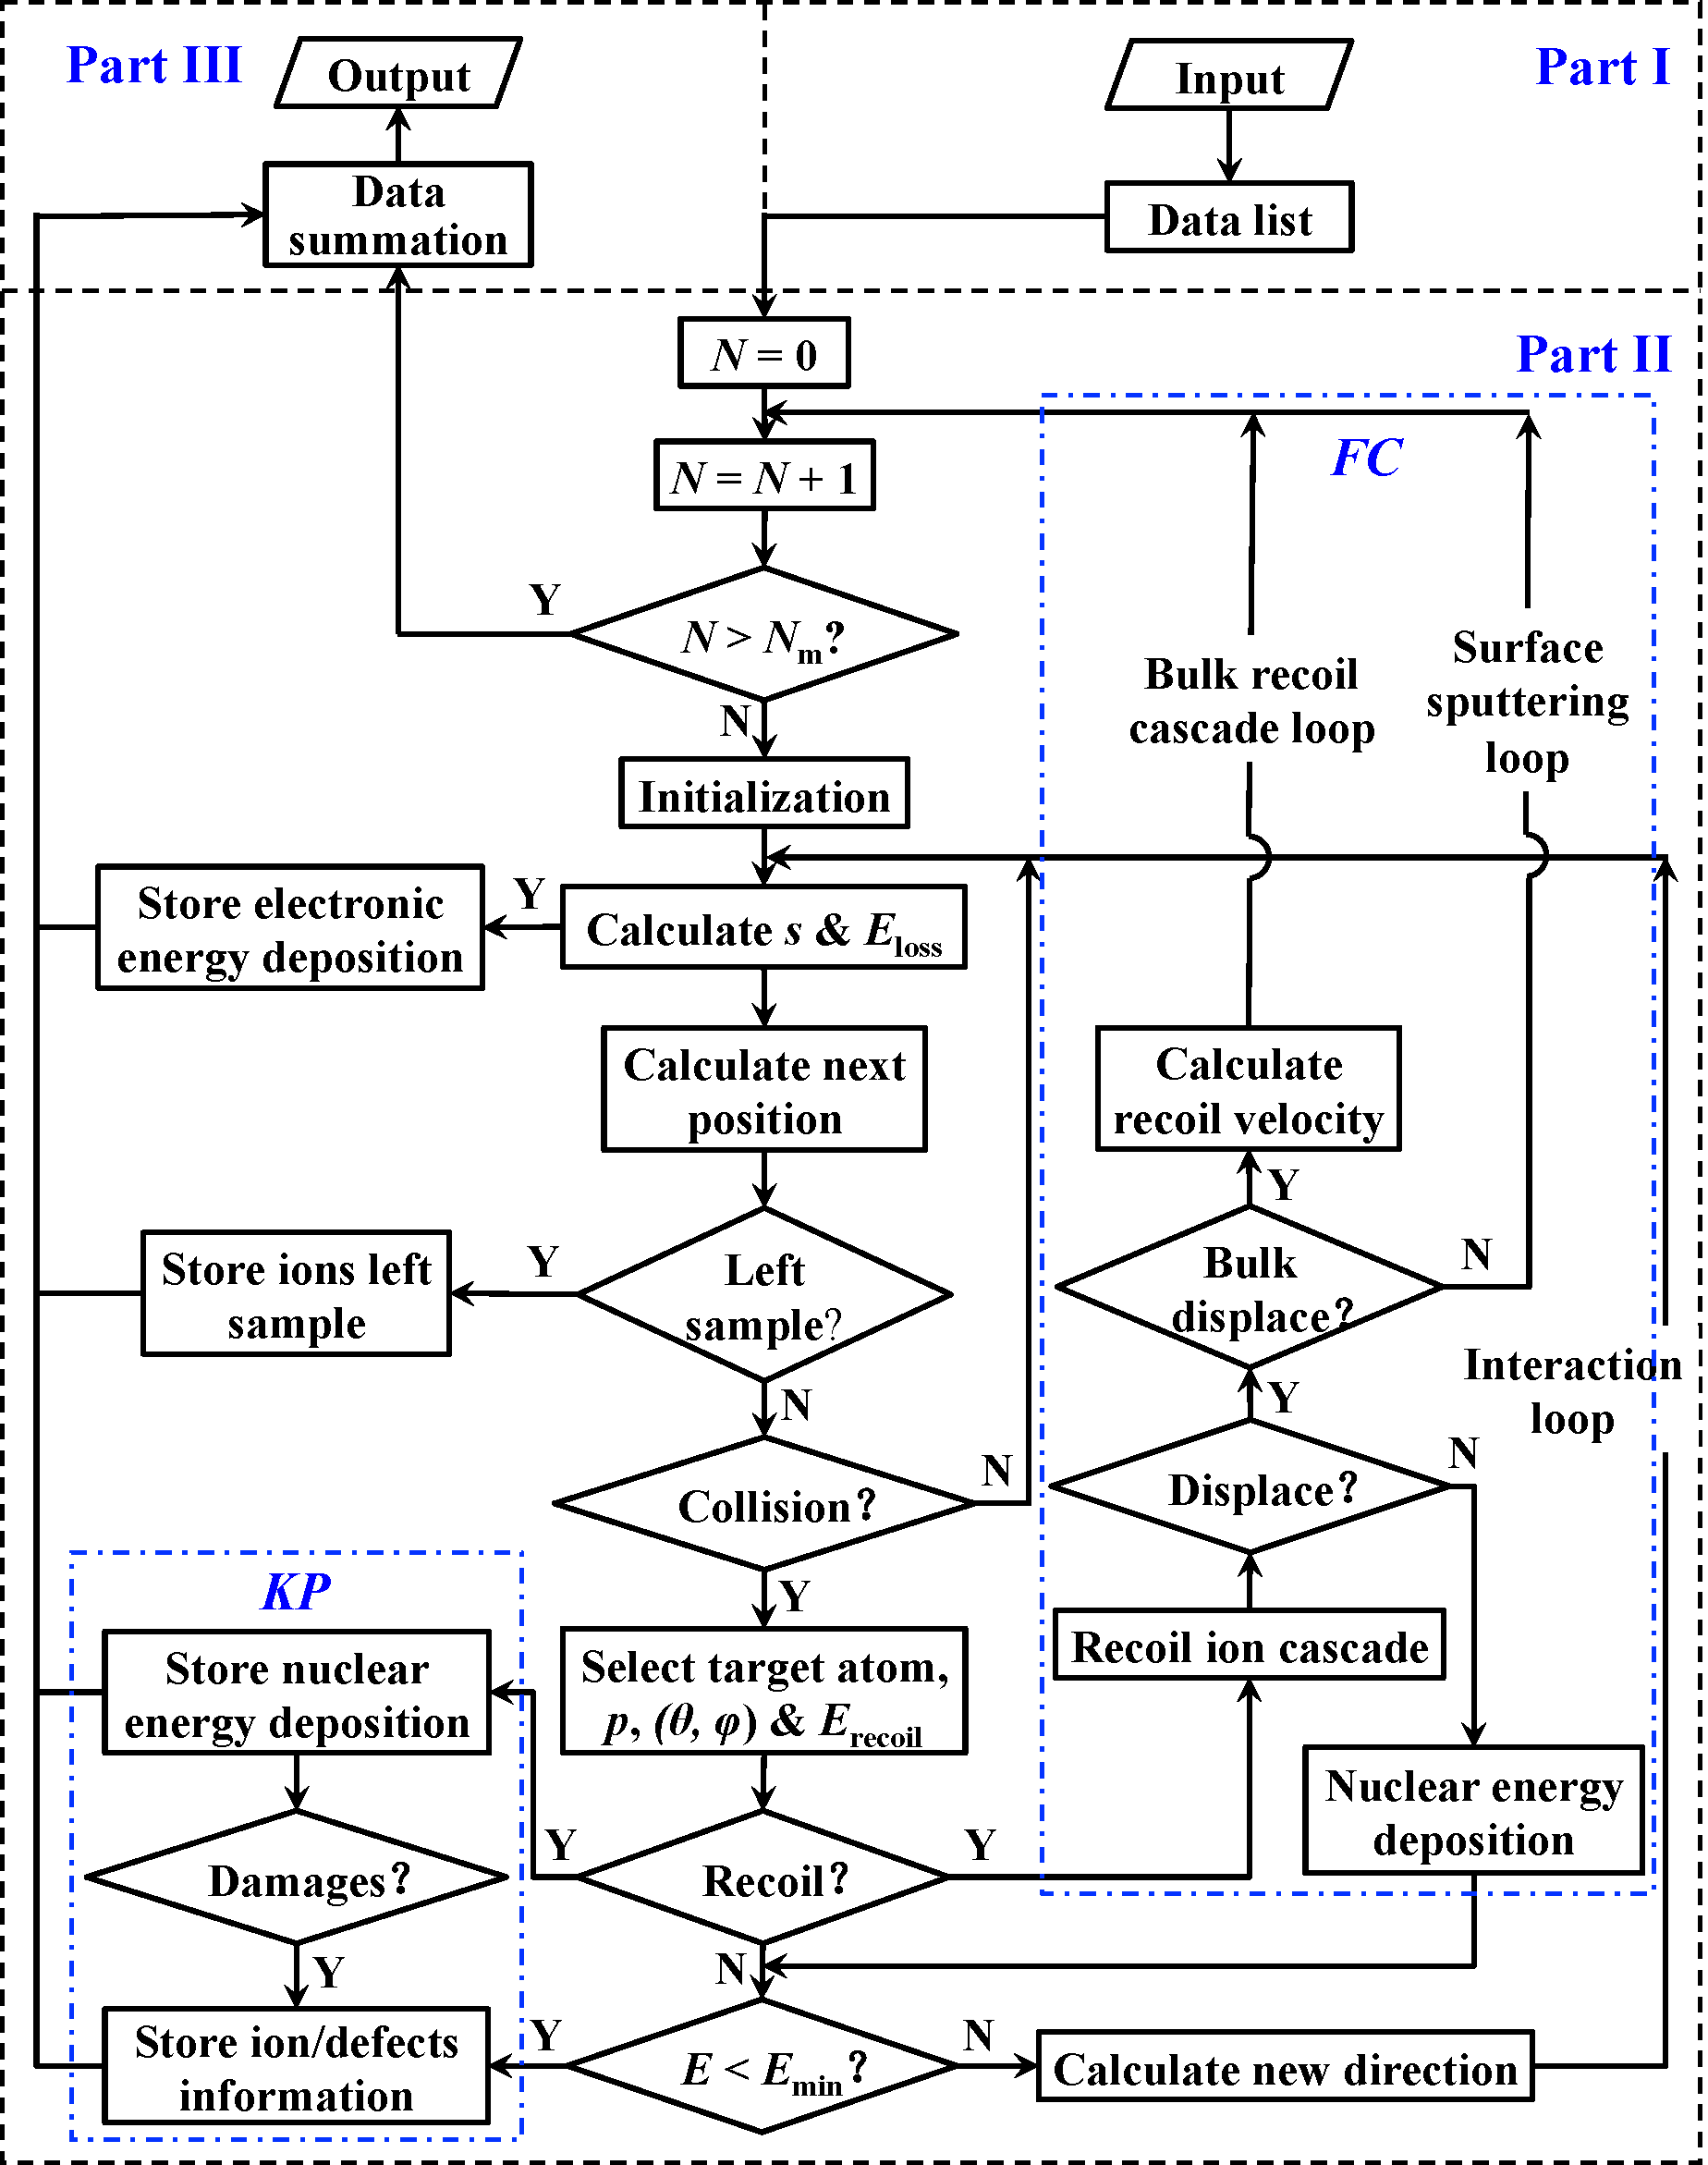
\includegraphics[width=0.68\textwidth]{fig1.pdf}
\caption{IM3D program chart of ions tracing and defects generation in a sample.} \label{Fig.1}
\end{figure}

For the elastic collision process, the classical binary atomic scattering angle $\theta_{CM}$ in the center-of-mass (CM) coordinate system can be evaluate accurately from the famous ``scattering integral" as,
\begin{equation}
\theta_{CM} = \pi - 2 \int_{r_0}^{\infty} \frac{p \cdot dr}{r^2 \sqrt{1 - \frac{V \left( r \right)}{E_c} - \left( \frac{p}{r} \right)^2}} \label{Eq.0}
\end{equation}
\noindent where, $p$ is the impact parameter, $r_0$ is the closet distance ($r$) between two atoms during the collision, $V\left( r \right)$ is the screened inter-atomic potential as listed below and $E_c$ is the kinetic energy of the incident atom in the center-of-mass frame. This integral can not be calculated analytically for inter-atomic screening potentials and hence a time-consuming numerical integration must be used instead\cite{Ziegler:2010}. An analytical approximation formula (such as the MAGIC approximation\cite{Ziegler:2010}) or a lookup table method (such as the fast indexing technique\cite{Schiettekatte:2008}) can be used in terms of accuracy and efficiency, as described in Section 2.3. The interaction potential $V \left( r \right)$ between two atoms is a screened repulsive Coulomb potential described by a dimensionless screening function, such as the Thomas-Feimi potential\cite{Sommerfeld:1932}, the Lenz-Jensen potential\cite{Lenz:1932}, the Moliere potential\cite{Moliere:1947}, the Bohr potential\cite{Bohr:1948} and the universal Ziggler-Biersack-Littmark (ZBL) potential\cite{Ziegler:2010}. In addition, the recoil energy of a target atom due to elastic nuclear collisions can be evaluated by the BCA between two charged particles involved in one scattering process.

For the inelastic collision process, the ion energy reduce uniformly along the free-flight-paths though the electronic energy losses accounting for the energy straggling. In IM3D code, the physical parameters such as electronic energy stopping powers are generated from SRModule.exe provided by SRIM package\cite{Ziegler:2004}, in the form of pre-calculated tables as implemented in Corteo\cite{Schiettekatte:2008}.
%In SRIM package (?), the Lindhard-Scharff formula for low energies and the Bethe-Bloch formula for high energies are used for evaluating electronic stopping cross sections, while the interpolation scheme is applied to provide a realistically smooth transition to bridge the gap between the low and high energy regions\cite{Biersack:1980}.
Either Bohr\cite{Bohr2:1948}, Chu\cite{Chu:1976} or Wang\cite{Yang:1991} formula can be selected to considering the energy straggling. Furthermore, IM3D code also employ a linear addition of stopping powers (known as Bragg's rule\cite{Bragg:1905}) for determining the stopping power in alloys, compounds and mixtures.

The generation of point defects (i.e. interstitials and vacancies) can be modeled by the analytical modified Kinchin-Pease (KP) model\cite{Kinchin:1955,Norgett:1975} or the computationally full cascade (FC) simulation.
%The modified KP model can only estimate the number of vacancies and assume the same local concentration for interstitials produced in a collision cascade, while the FC simulation can accurately determine the location of the interstitials by tracing the trajectories of all recoiling atoms in a collision cascade but requires a greater computational effort.
%By comparing to NRT and MD calculation results, Stroller et. al pointed out that it is recommended that when direct comparisons between ion and neutron data are intended, the KP option of SRIM code should be selected\cite{Stoller:2013}.
Assume a trajectory atom with atomic number $Z_1$ and energy $E$ collide with a target atom with atomic number $Z_2$. After the collision event, the energy of the trajectory atom change to $E_1$ and the target atom obtains energy $E_2$, and thus different damage generation processes would also occur: (1) if $E_2 > E_d$ ($E_d$ is the displacement energy of the target atom), a displacement occurs so that the target atom has enough energy to leave the site; (2) if both $E_1 > E_d$ and $E_2 > E_d$, a vacancy occurs; (3) if $E_2 < E_d$, the target atom without enough energy will vibrate back to its site releasing energy $E_2$ as phonons; (4) if $E_1 < E_b$ ($E_b$ is the lattice/surface binding energy of the target atom), $E_2 > E_d$ and $Z_1 = Z_2$, a replacement collision occurs with energy $E_1$ releasing as phonons; (5) if ($E_1 < E_{min}~or~E_b$, $E_2 > E_d$ and $Z_1 \neq Z_2$) or ($E_1 < E_{min}~or~E_b$ and $E_2 < E_d$), the trajectory atom becomes an interstitial atom.

% Appendix A

\chapter{3D structural models} % Main appendix title

\label{AppendixB} % For referencing this appendix elsewhere, use \ref{AppendixA}

\lhead{Appendix B. \emph{3D structural models}} % This is for the header on each page - perhaps a shortened title

The arbitrary complex 3D nanostructured targets can be generated by graphical softwares beforehand and traced by two types of sophisticated 3D structural algorithms in IM3D code, that is, CSG and FETM methods\cite{Li2:2011,Li:2013}. Then the different types of targets are set in the corresponding coordinate systems as shown in Fig.\ref{Fig.2}, respectively. The ion beams with different atomic numbers and incident directions follow different types of space-distributions (i.e., specified point, center point, uniform or Gaussian random distributions and so on). The targets are considered as composing of different geometric elements each of which with different amorphous materials (i.e., elements, alloys and compounds).

\begin{figure}[!ht]\centering
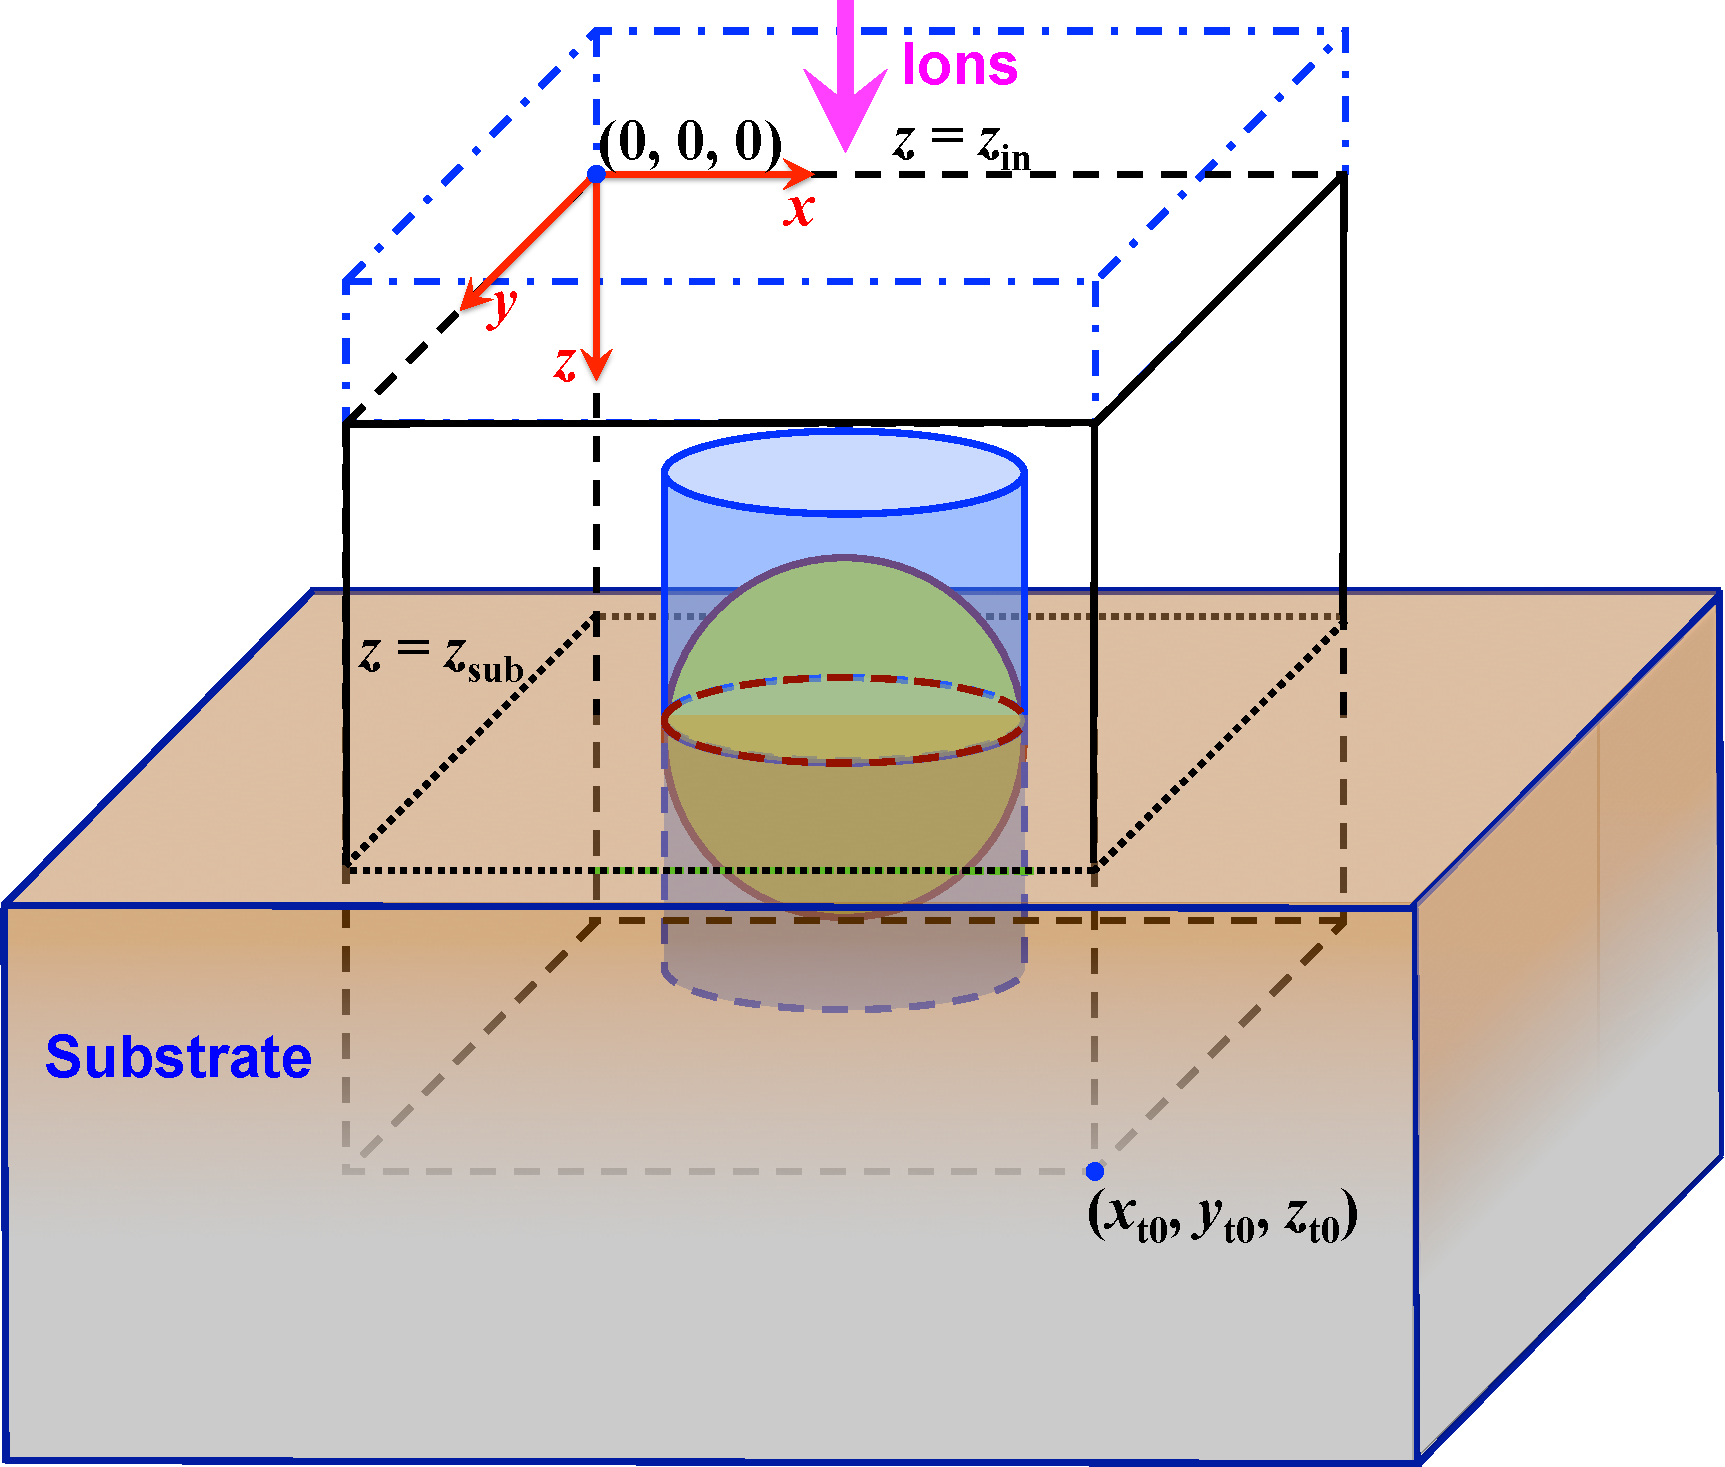
\includegraphics[width=0.48\textwidth]{fig2-a.pdf}
%\label{Fig.1a}
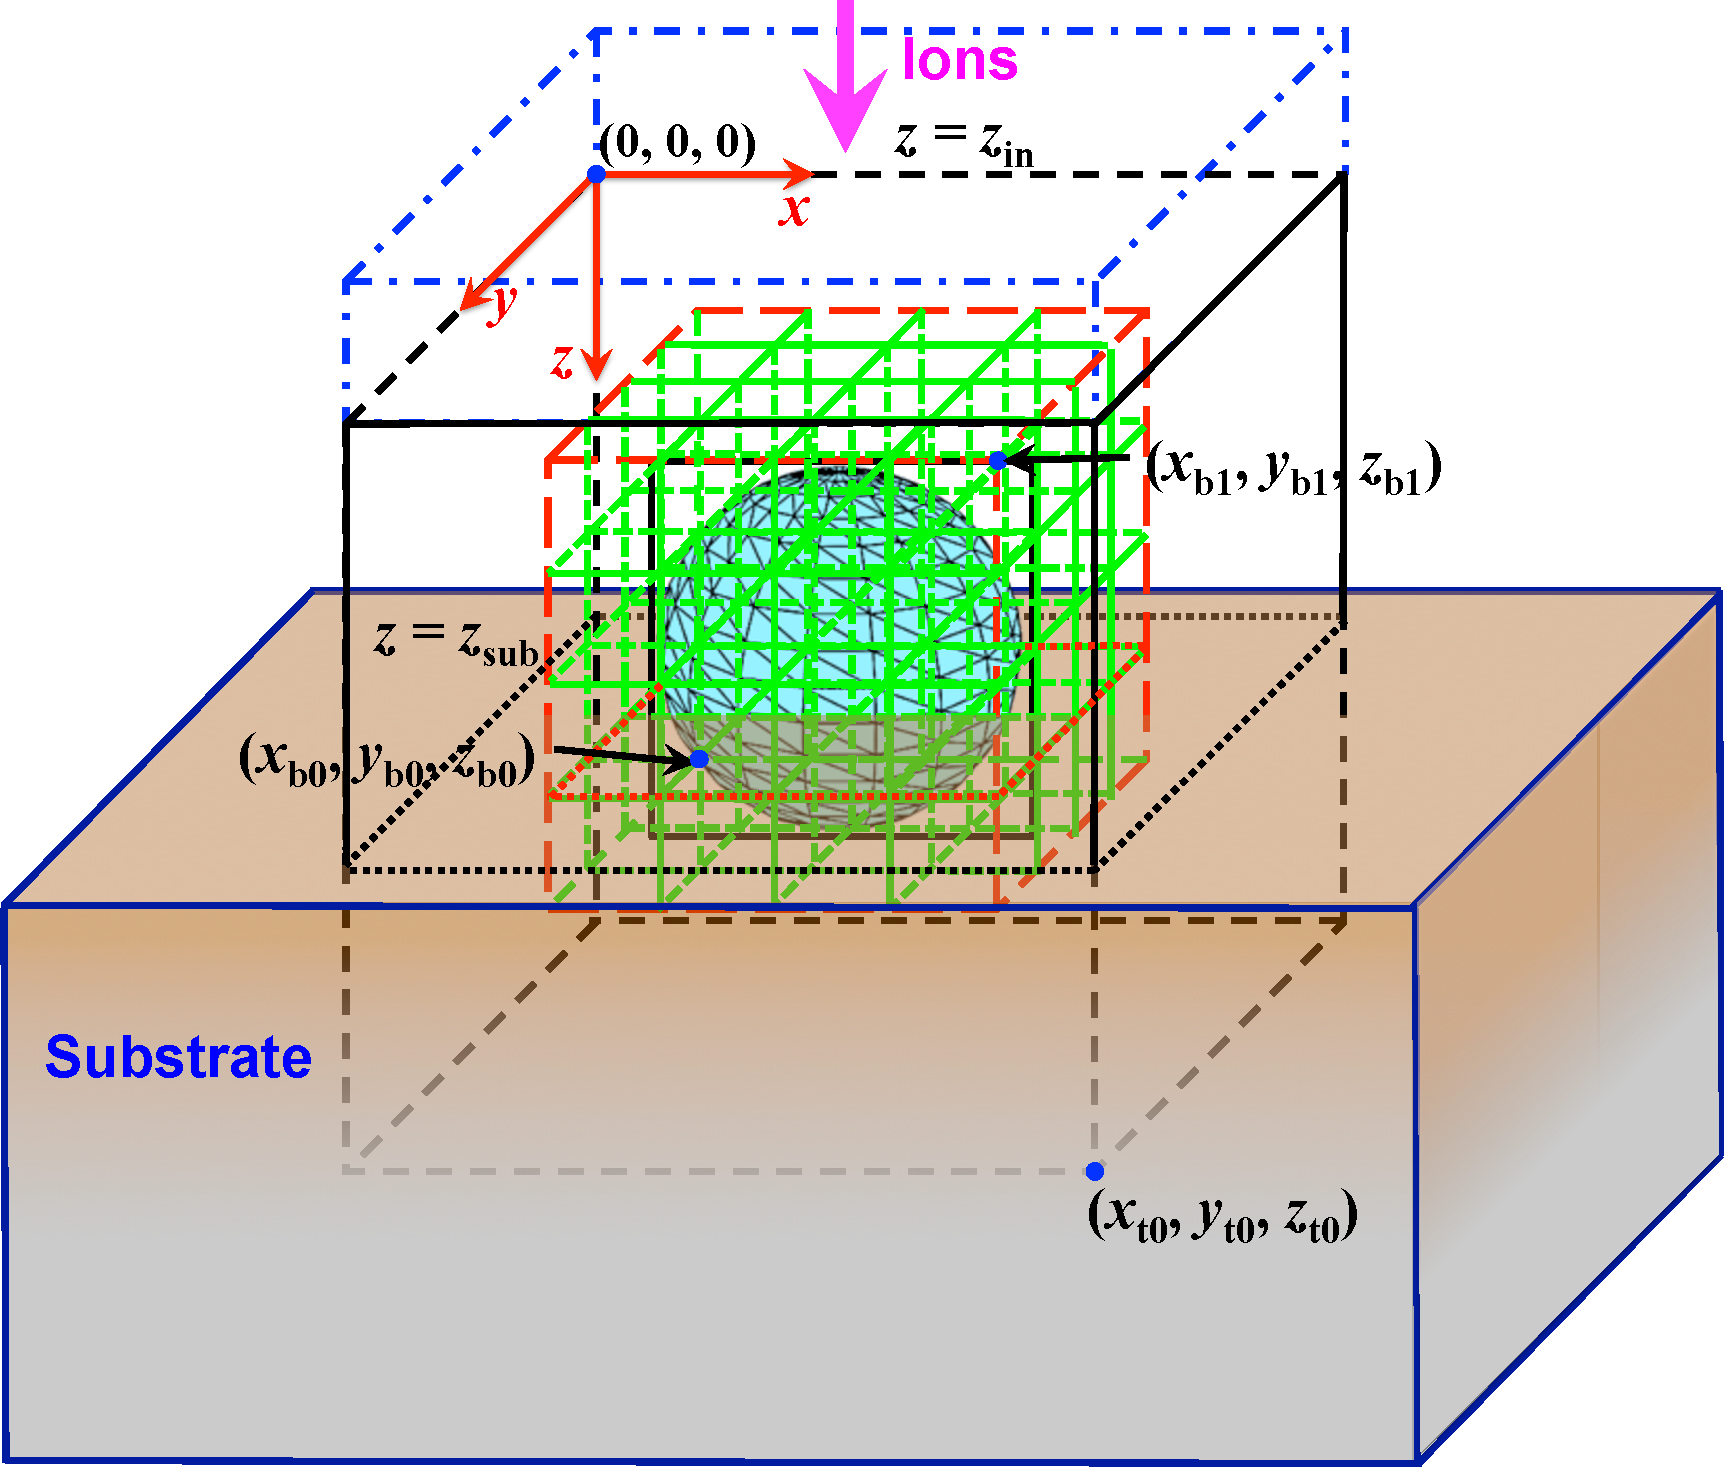
\includegraphics[width=0.48\textwidth]{fig2-b.pdf}
%\label{Fig.1b}
\caption{CSG and FETM geometric models and the corresponding coordinate systems.} \label{Fig.2}
\end{figure}

On the one hand, CSG method\cite{Li:2005,Li:2009} is simply introduced in IM3D code which uses simple geometries to build a complex structure with Boolean operations: union, difference and intersection, etc. By CSG modeling, a complex geometric structure can be constructed with some basic and simple 3D bodies as elements that can be analytically described with a few parameters. The basic elements, such as sphere, tetrahedron, cuboid, ellipsoid, taper, column, polyhedron, paraboloid, hyperboloid and so on, can be easily implemented into subroutines to allow efficient calculation of intersecting points of an ion trajectory with a geometric surface. Detailed construction process can be found in Refs.\cite{Li:2005,Li:2009} . The limits of this method are mainly from two sides: firstly, it is obvious that, with the limited number of parameters, one cannot in practice build an arbitrary-complex geometric structures. Fortunately, most of the simple geometric nanostructures can be modeled by the present algorithm. Secondly, for the step of ion/atom trajectories, one has to compute the intersection points with every possible basic shape. A large number of such judging procedures in a MC simulation would cause a heavy computing cost. An efficient parallel algorithm is needed for the simulation of very complex targets constructing with this geometric model.

On the other hand, FETM method\cite{Li:2008,Zhang:2011} in computer graphics is also employed in IM3D code by using a finite element triangle mesh to construct a sample surface, and furthermore, by using the space subdivision method to accelerate the calculation. In principle, it allows an easy construction of an arbitrary-complex geometric structure with smooth or roughness surface. A closed 3D geometric structure can be constructed by just joining a series of mesh points that outline the 3D geometric structure, which can be generated easily by different algorithms with different graphical softwares (such as Gmsh software\cite{Geuzaine:2009}) or even user's own definition. The accepted formats of FETM shape files are $opengl$ and $ply2$ at present. The reason to use a triangulated mesh is due to its advantage on easier judging of intersection points of a velocity vector with a local triangular plane when considering an ion incidence into a sample surface or emission from a surface. This method is more realistic and unified for simulating much complex targets while on the premise of spending less consuming time.

In IM3D code, the trajectories are traced step by step in a complex 3D target. The free-flight-paths of an ion between two successive collision events follow the Poisson distribution with a mean free-flight-path of $l = n^{(-1/3)}$ (where $n$ is the atomic density of the target) or a constant value specified by user. Afterwards, a ray-tracing technique\cite{Li:2005,Li:2009} for an inhomogeneous specimen with a complex geometric structure and the space subdivision method are introduced to accelerate the calculations\cite{Li:2008,Zhang:2011}. Furthermore, when ions transport in a specimen, three physical quantities, i.e. the free-flight-path, the direction deflection, and the kinetic energy change after refraction at surface/interface, must be treated appropriately, especially at the boundaries of complex geometric structures\cite{Li:2008}.

%% Appendix A

\chapter{xxxx} % Main appendix title

\label{AppendixA} % For referencing this appendix elsewhere, use \ref{AppendixA}

\lhead{Appendix A. \emph{xxxx}} % This is for the header on each page - perhaps a shortened title



\addtocontents{toc}{\vspace{2em}} % Add a gap in the Contents, for aesthetics

\backmatter

%----------------------------------------------------------------------------------------
%	BIBLIOGRAPHY
%----------------------------------------------------------------------------------------

\label{Bibliography}

\lhead{\emph{Bibliography}} % Change the page header to say "Bibliography"

\bibliographystyle{unsrtnat} % Use the "unsrtnat" BibTeX style for formatting the Bibliography

\bibliography{Bibliography} % The references (bibliography) information are stored in the file named "Bibliography.bib"

\end{document}